\documentclass{article}

% Hier befinden sich Pakete, die wir beinahe immer benutzen ...

\usepackage[utf8]{inputenc}

% Sprach-Paket:
\usepackage[ngerman]{babel}

% damit's nicht so, wie beim Grill aussieht:
\usepackage{fullpage}

% Mathematik:
\usepackage{amsmath, amssymb, amsfonts, amsthm}
\usepackage{bbm}
\usepackage{mathtools, mathdots}

% Makros mit mehereren Default-Argumenten:
\usepackage{twoopt}

% Anführungszeichen (Makro \Quote{}):
\usepackage{babel}

% if's für Makros:
\usepackage{xifthen}
\usepackage{etoolbox}

% tikz ist kein Zeichenprogramm (doch!):
\usepackage{tikz}

% bessere Aufzählungen:
\usepackage{enumitem}

% (bessere) Umgebung für Bilder:
\usepackage{graphicx, subfig, float}

% Umgebung für Code:
\usepackage{listings}

% Farben:
\usepackage{xcolor}

% Umgebung für "plain text":
\usepackage{verbatim}

% Umgebung für mehrerer Spalten:
\usepackage{multicol}

% "nette" Brüche
\usepackage{nicefrac}

% Spaltentypen verschiedener Dicke
\usepackage{tabularx}
\usepackage{makecell}

% Für Vektoren
\usepackage{esvect}

% (Web-)Links
\usepackage{hyperref}

% Zitieren & Literatur-Verzeichnis
\usepackage[style = authoryear]{biblatex}
\usepackage{csquotes}

% so ähnlich wie mathbb
%\usepackage{mathds}

% Keine Ahnung, was das macht ...
\usepackage{booktabs}
\usepackage{ngerman}
\usepackage{placeins}

% special letters:

\newcommand{\N}{\mathbb{N}}
\newcommand{\Z}{\mathbb{Z}}
\newcommand{\Q}{\mathbb{Q}}
\newcommand{\R}{\mathbb{R}}
\newcommand{\C}{\mathbb{C}}
\newcommand{\K}{\mathbb{K}}
\newcommand{\T}{\mathbb{T}}
\newcommand{\E}{\mathbb{E}}
\newcommand{\V}{\mathbb{V}}
\renewcommand{\S}{\mathbb{S}}
\renewcommand{\P}{\mathbb{P}}
\newcommand{\1}{\mathbbm{1}}

% quantors:

\newcommand{\Forall}{\forall \,}
\newcommand{\Exists}{\exists \,}
\newcommand{\ExistsOnlyOne}{\exists! \,}
\newcommand{\nExists}{\nexists \,}
\newcommand{\ForAlmostAll}{\forall^\infty \,}

% MISC symbols:

\newcommand{\landau}{{\scriptstyle \mathcal{O}}}
\newcommand{\Landau}{\mathcal{O}}


\newcommand{\eps}{\mathrm{eps}}

% graphics in a box:

\newcommandtwoopt
{\includegraphicsboxed}[3][][]
{
  \begin{figure}[!h]
    \begin{boxedin}
      \ifthenelse{\isempty{#1}}
      {
        \begin{center}
          \includegraphics[width = 0.75 \textwidth]{#3}
          \label{fig:#2}
        \end{center}
      }{
        \begin{center}
          \includegraphics[width = 0.75 \textwidth]{#3}
          \caption{#1}
          \label{fig:#2}
        \end{center}
      }
    \end{boxedin}
  \end{figure}
}

% braces:

\newcommand{\pbraces}[1]{{\left  ( #1 \right  )}}
\newcommand{\bbraces}[1]{{\left  [ #1 \right  ]}}
\newcommand{\Bbraces}[1]{{\left \{ #1 \right \}}}
\newcommand{\vbraces}[1]{{\left  | #1 \right  |}}
\newcommand{\Vbraces}[1]{{\left \| #1 \right \|}}
\newcommand{\abraces}[1]{{\left \langle #1 \right \rangle}}
\newcommand{\round}[1]{\bbraces{#1}}

\newcommand
{\floorbraces}[1]
{{\left \lfloor #1 \right \rfloor}}

\newcommand
{\ceilbraces} [1]
{{\left \lceil  #1 \right \rceil }}

% special functions:

\newcommand{\norm}  [2][]{\Vbraces{#2}_{#1}}
\newcommand{\diam}  [2][]{\mathrm{diam}_{#1} \: #2}
\newcommand{\diag}  [1]{\mathrm{diag} \: #1}
\newcommand{\dist}  [1]{\mathrm{dist} \: #1}
\newcommand{\mean}  [1]{\mathrm{mean} \: #1}
\newcommand{\erf}   [1]{\mathrm{erf} \: #1}
\newcommand{\id}    [1]{\mathrm{id} \: #1}
\newcommand{\sgn}   [1]{\mathrm{sgn} \: #1}
\newcommand{\supp}  [1]{\mathrm{supp} \: #1}
\newcommand{\arsinh}[1]{\mathrm{arsinh} \: #1}
\newcommand{\arcosh}[1]{\mathrm{arcosh} \: #1}
\newcommand{\artanh}[1]{\mathrm{artanh} \: #1}
\newcommand{\card}  [1]{\mathrm{card} \: #1}
\newcommand{\Span}  [1]{\mathrm{span} \: #1}
\newcommand{\Aut}   [1]{\mathrm{Aut} \: #1}
\newcommand{\End}   [1]{\mathrm{End} \: #1}
\newcommand{\ggT}   [1]{\mathrm{ggT} \: #1}
\newcommand{\kgV}   [1]{\mathrm{kgV} \: #1}
\newcommand{\ord}   [1]{\mathrm{ord} \: #1}
\newcommand{\grad}  [1]{\mathrm{grad} \: #1}
\newcommand{\ran}   [1]{\mathrm{ran} \: #1}
\newcommand{\graph} [1]{\mathrm{graph} \: #1}
\newcommand{\Inv}   [1]{\mathrm{Inv} \: #1}
\newcommand{\pv}    [1]{\mathrm{pv} \: #1}
\newcommand{\GL}    [1]{\mathrm{GL} \: #1}
\newcommand{\Mod}{\mathrm{Mod} \:}
\newcommand{\Th}{\mathrm{Th} \:}
\newcommand{\Char}{\mathrm{char}}
\newcommand{\At}{\mathrm{At}}
\newcommand{\Ob}{\mathrm{Ob}}
\newcommand{\Hom}{\mathrm{Hom}}
\newcommand{\orthogonal}[3][]{#2 ~\bot_{#1}~ #3}
\newcommand{\Rang}{\mathrm{Rang}}
\newcommand{\NIL}{\mathrm{NIL}}
\newcommand{\Res}{\mathrm{Res}}
\newcommand{\lxor}{\dot \lor}
\newcommand{\Div}{\mathrm{div} \:}
\newcommand{\meas}{\mathrm{meas} \:}

% fractions:

\newcommand{\Frac}[2]{\frac{1}{#1} \pbraces{#2}}
\newcommand{\nfrac}[2]{\nicefrac{#1}{#2}}

% derivatives & integrals:

\newcommandtwoopt
{\Int}[4][][]
{\int_{#1}^{#2} #3 ~\mathrm{d} #4}

\newcommandtwoopt
{\derivative}[3][][]
{
  \frac
  {\mathrm{d}^{#1} #2}
  {\mathrm{d} #3^{#1}}
}

\newcommandtwoopt
{\pderivative}[3][][]
{
  \frac
  {\partial^{#1} #2}
  {\partial #3^{#1}}
}

\newcommand
{\primeprime}
{{\prime \prime}}

\newcommand
{\primeprimeprime}
{{\prime \prime \prime}}

% Text:

\newcommand{\Quote}[1]{\glqq #1\grqq{}}
\newcommand{\Text}[1]{{\text{#1}}}
\newcommand{\fastueberall}{\text{f.ü.}}
\newcommand{\fastsicher}{\text{f.s.}}

% -------------------------------- %
% amsthm-stuff:

\theoremstyle{definition}

% numbered theorems
\newtheorem{theorem}{Satz}
\newtheorem{lemma}{Lemma}
\newtheorem{corollary}{Korollar}
\newtheorem{proposition}{Proposition}
\newtheorem{remark}{Bemerkung}
\newtheorem{definition}{Definition}
\newtheorem{example}{Beispiel}

% unnumbered theorems
\newtheorem*{theorem*}{Satz}
\newtheorem*{lemma*}{Lemma}
\newtheorem*{corollary*}{Korollar}
\newtheorem*{proposition*}{Proposition}
\newtheorem*{remark*}{Bemerkung}
\newtheorem*{definition*}{Definition}
\newtheorem*{example*}{Beispiel}

% Please define this stuff in project ("main.tex"):

% \def \lastexercisenumber {...}
% This will be 0 by default

% \setcounter{section}{...}
% This will be 0 by default
% and hence, completely ignored

\ifnum \thesection = 0
{\newtheorem{exercise}{Aufgabe}}
\else
{\newtheorem{exercise}{Aufgabe}[section]}
\fi

\ifdef
{\lastexercisenumber}
{\setcounter{exercise}{\lastexercisenumber}}

\newcommand{\solution}
{
    \renewcommand{\proofname}{Lösung}
    \renewcommand{\qedsymbol}{}
    \proof
}

\renewcommand{\proofname}{Beweis}

% -------------------------------- %
% environment zum einkasteln:

% dickere vertical lines
\newcolumntype
{x}
[1]
{!{\centering\arraybackslash\vrule width #1}}

% environment selbst (the big cheese)
\newenvironment
{boxedin}
{
  \begin{tabular}
  {
    x{1 pt}
    p{\textwidth}
    x{1 pt}
  }
  \Xhline
  {2 \arrayrulewidth}
}
{
  \\
  \Xhline{2 \arrayrulewidth}
  \end{tabular}
}

% -------------------------------- %
% MISC "Ein-Deutschungen"

\renewcommand
{\figurename}
{Abbildung}

\renewcommand
{\tablename}
{Tabelle}

% -------------------------------- %

% ---------------------------------------------------------------- %
% https://www.overleaf.com/learn/latex/Code_listing

\definecolor{codegreen} {rgb}{0, 0.6, 0}
\definecolor{codegray}    {rgb}{0.5, 0.5, 0.5}
\definecolor{codepurple}{rgb}{0.58, 0, 0.82}
\definecolor{backcolour}{rgb}{0.95, 0.95, 0.92}

\lstdefinestyle{overleaf}
{
    backgroundcolor = \color{backcolour},
    commentstyle = \color{codegreen},
    keywordstyle = \color{magenta},
    numberstyle = \tiny\color{codegray},
    stringstyle = \color{codepurple},
    basicstyle = \ttfamily \footnotesize,
    breakatwhitespace = false,
    breaklines = true,
    captionpos = b,
    keepspaces = true,
    numbers = left,
    numbersep = 5pt,
    showspaces = false,
    showstringspaces = false,
    showtabs = false,
    tabsize = 2
}

% ---------------------------------------------------------------- %
% https://en.wikibooks.org/wiki/LaTeX/Source_Code_Listings

\lstdefinestyle{customc}
{
    belowcaptionskip = 1 \baselineskip,
    breaklines = true,
    frame = L,
    xleftmargin = \parindent,
    language = C,
    showstringspaces = false,
    basicstyle = \footnotesize \ttfamily,
    keywordstyle = \bfseries \color{green!40!black},
    commentstyle = \itshape \color{purple!40!black},
    identifierstyle = \color{blue},
    stringstyle = \color{orange},
}

\lstdefinestyle{customasm}
{
    belowcaptionskip = 1 \baselineskip,
    frame = L,
    xleftmargin = \parindent,
    language = [x86masm] Assembler,
    basicstyle = \footnotesize\ttfamily,
    commentstyle = \itshape\color{purple!40!black},
}

% ---------------------------------------------------------------- %
% https://tex.stackexchange.com/questions/235731/listings-syntax-for-literate

\definecolor{maroon}        {cmyk}{0, 0.87, 0.68, 0.32}
\definecolor{halfgray}      {gray}{0.55}
\definecolor{ipython_frame} {RGB}{207, 207, 207}
\definecolor{ipython_bg}    {RGB}{247, 247, 247}
\definecolor{ipython_red}   {RGB}{186, 33, 33}
\definecolor{ipython_green} {RGB}{0, 128, 0}
\definecolor{ipython_cyan}  {RGB}{64, 128, 128}
\definecolor{ipython_purple}{RGB}{170, 34, 255}

\lstdefinestyle{stackexchangePython}
{
    breaklines = true,
    %
    extendedchars = true,
    literate =
    {á}{{\' a}} 1 {é}{{\' e}} 1 {í}{{\' i}} 1 {ó}{{\' o}} 1 {ú}{{\' u}} 1
    {Á}{{\' A}} 1 {É}{{\' E}} 1 {Í}{{\' I}} 1 {Ó}{{\' O}} 1 {Ú}{{\' U}} 1
    {à}{{\` a}} 1 {è}{{\` e}} 1 {ì}{{\` i}} 1 {ò}{{\` o}} 1 {ù}{{\` u}} 1
    {À}{{\` A}} 1 {È}{{\' E}} 1 {Ì}{{\` I}} 1 {Ò}{{\` O}} 1 {Ù}{{\` U}} 1
    {ä}{{\" a}} 1 {ë}{{\" e}} 1 {ï}{{\" i}} 1 {ö}{{\" o}} 1 {ü}{{\" u}} 1
    {Ä}{{\" A}} 1 {Ë}{{\" E}} 1 {Ï}{{\" I}} 1 {Ö}{{\" O}} 1 {Ü}{{\" U}} 1
    {â}{{\^ a}} 1 {ê}{{\^ e}} 1 {î}{{\^ i}} 1 {ô}{{\^ o}} 1 {û}{{\^ u}} 1
    {Â}{{\^ A}} 1 {Ê}{{\^ E}} 1 {Î}{{\^ I}} 1 {Ô}{{\^ O}} 1 {Û}{{\^ U}} 1
    {œ}{{\oe}}  1 {Œ}{{\OE}}  1 {æ}{{\ae}}  1 {Æ}{{\AE}}  1 {ß}{{\ss}}  1
    {ç}{{\c c}} 1 {Ç}{{\c C}} 1 {ø}{{\o}} 1 {å}{{\r a}} 1 {Å}{{\r A}} 1
    {€}{{\EUR}} 1 {£}{{\pounds}} 1
}


% Python definition (c) 1998 Michael Weber
% Additional definitions (2013) Alexis Dimitriadis
% modified by me (should not have empty lines)

\lstdefinelanguage{iPython}{
    morekeywords = {access, and, break, class, continue, def, del, elif, else, except, exec, finally, for, from, global, if, import, in, is, lambda, not, or, pass, print, raise, return, try, while}, %
    %
    % Built-ins
    morekeywords = [2]{abs, all, any, basestring, bin, bool, bytearray, callable, chr, classmethod, cmp, compile, complex, delattr, dict, dir, divmod, enumerate, eval, execfile, file, filter, float, format, frozenset, getattr, globals, hasattr, hash, help, hex, id, input, int, isinstance, issubclass, iter, len, list, locals, long, map, max, memoryview, min, next, object, oct, open, ord, pow, property, range, raw_input, reduce, reload, repr, reversed, round, set, setattr, slice, sorted, staticmethod, str, sum, super, tuple, type, unichr, unicode, vars, xrange, zip, apply, buffer, coerce, intern}, %
    %
    sensitive = true, %
    morecomment = [l] \#, %
    morestring = [b]', %
    morestring = [b]", %
    %
    morestring = [s]{'''}{'''}, % used for documentation text (mulitiline strings)
    morestring = [s]{"""}{"""}, % added by Philipp Matthias Hahn
    %
    morestring = [s]{r'}{'},     % `raw' strings
    morestring = [s]{r"}{"},     %
    morestring = [s]{r'''}{'''}, %
    morestring = [s]{r"""}{"""}, %
    morestring = [s]{u'}{'},     % unicode strings
    morestring = [s]{u"}{"},     %
    morestring = [s]{u'''}{'''}, %
    morestring = [s]{u"""}{"""}, %
    %
    % {replace}{replacement}{lenght of replace}
    % *{-}{-}{1} will not replace in comments and so on
    literate = 
    {á}{{\' a}} 1 {é}{{\' e}} 1 {í}{{\' i}} 1 {ó}{{\' o}} 1 {ú}{{\' u}} 1
    {Á}{{\' A}} 1 {É}{{\' E}} 1 {Í}{{\' I}} 1 {Ó}{{\' O}} 1 {Ú}{{\' U}} 1
    {à}{{\` a}} 1 {è}{{\` e}} 1 {ì}{{\` i}} 1 {ò}{{\` o}} 1 {ù}{{\` u}} 1
    {À}{{\` A}} 1 {È}{{\' E}} 1 {Ì}{{\` I}} 1 {Ò}{{\` O}} 1 {Ù}{{\` U}} 1
    {ä}{{\" a}} 1 {ë}{{\" e}} 1 {ï}{{\" i}} 1 {ö}{{\" o}} 1 {ü}{{\" u}} 1
    {Ä}{{\" A}} 1 {Ë}{{\" E}} 1 {Ï}{{\" I}} 1 {Ö}{{\" O}} 1 {Ü}{{\" U}} 1
    {â}{{\^ a}} 1 {ê}{{\^ e}} 1 {î}{{\^ i}} 1 {ô}{{\^ o}} 1 {û}{{\^ u}} 1
    {Â}{{\^ A}} 1 {Ê}{{\^ E}} 1 {Î}{{\^ I}} 1 {Ô}{{\^ O}} 1 {Û}{{\^ U}} 1
    {œ}{{\oe}}  1 {Œ}{{\OE}}  1 {æ}{{\ae}}  1 {Æ}{{\AE}}  1 {ß}{{\ss}}  1
    {ç}{{\c c}} 1 {Ç}{{\c C}} 1 {ø}{{\o}} 1 {å}{{\r a}} 1 {Å}{{\r A}} 1
    {€}{{\EUR}} 1 {£}{{\pounds}} 1
    %
    {^}{{{\color{ipython_purple}\^ {}}}} 1
    { = }{{{\color{ipython_purple} = }}} 1
    %
    {+}{{{\color{ipython_purple}+}}} 1
    {*}{{{\color{ipython_purple}$^\ast$}}} 1
    {/}{{{\color{ipython_purple}/}}} 1
    %
    {+=}{{{+=}}} 1
    {-=}{{{-=}}} 1
    {*=}{{{$^\ast$ = }}} 1
    {/=}{{{/=}}} 1,
    literate = 
    *{-}{{{\color{ipython_purple} -}}} 1
     {?}{{{\color{ipython_purple} ?}}} 1,
    %
    identifierstyle = \color{black}\ttfamily,
    commentstyle = \color{ipython_cyan}\ttfamily,
    stringstyle = \color{ipython_red}\ttfamily,
    keepspaces = true,
    showspaces = false,
    showstringspaces = false,
    %
    rulecolor = \color{ipython_frame},
    frame = single,
    frameround = {t}{t}{t}{t},
    framexleftmargin = 6mm,
    numbers = left,
    numberstyle = \tiny\color{halfgray},
    %
    %
    backgroundcolor = \color{ipython_bg},
    % extendedchars = true,
    basicstyle = \scriptsize,
    keywordstyle = \color{ipython_green}\ttfamily,
}

% ---------------------------------------------------------------- %
% https://tex.stackexchange.com/questions/417884/colour-r-code-to-match-knitr-theme-using-listings-minted-or-other

\geometry{verbose, tmargin = 2.5cm, bmargin = 2.5cm, lmargin = 2.5cm, rmargin = 2.5cm}

\definecolor{backgroundCol}  {rgb}{.97, .97, .97}
\definecolor{commentstyleCol}{rgb}{0.678, 0.584, 0.686}
\definecolor{keywordstyleCol}{rgb}{0.737, 0.353, 0.396}
\definecolor{stringstyleCol} {rgb}{0.192, 0.494, 0.8}
\definecolor{NumCol}         {rgb}{0.686, 0.059, 0.569}
\definecolor{basicstyleCol}  {rgb}{0.345, 0.345, 0.345}

\lstdefinestyle{stackexchangeR}
{
    language = R,                                        % the language of the code
    basicstyle = \small \ttfamily \color{basicstyleCol}, % the size of the fonts that are used for the code
    % numbers = left,                                      % where to put the line-numbers
    numberstyle = \color{green},                         % the style that is used for the line-numbers
    stepnumber = 1,                                      % the step between two line-numbers. If it is 1, each line will be numbered
    numbersep = 5pt,                                     % how far the line-numbers are from the code
    backgroundcolor = \color{backgroundCol},             % choose the background color. You must add \usepackage{color}
    showspaces = false,                                  % show spaces adding particular underscores
    showstringspaces = false,                            % underline spaces within strings
    showtabs = false,                                    % show tabs within strings adding particular underscores
    % frame = single,                                      % adds a frame around the code
    % rulecolor = \color{white},                           % if not set, the frame-color may be changed on line-breaks within not-black text (e.g. commens (green here))
    tabsize = 2,                                         % sets default tabsize to 2 spaces
    captionpos = b,                                      % sets the caption-position to bottom
    breaklines = true,                                   % sets automatic line breaking
    breakatwhitespace = false,                           % sets if automatic breaks should only happen at whitespace
    keywordstyle = \color{keywordstyleCol},              % keyword style
    commentstyle = \color{commentstyleCol},              % comment style
    stringstyle = \color{stringstyleCol},                % string literal style
    literate = %
    *{0}{{{\color{NumCol} 0}}} 1
     {1}{{{\color{NumCol} 1}}} 1
     {2}{{{\color{NumCol} 2}}} 1
     {3}{{{\color{NumCol} 3}}} 1
     {4}{{{\color{NumCol} 4}}} 1
     {5}{{{\color{NumCol} 5}}} 1
     {6}{{{\color{NumCol} 6}}} 1
     {7}{{{\color{NumCol} 7}}} 1
     {8}{{{\color{NumCol} 8}}} 1
     {9}{{{\color{NumCol} 9}}} 1
}

% ---------------------------------------------------------------- %
% Fundament Mathematik

\lstdefinestyle{fundament}{basicstyle = \ttfamily}

% ---------------------------------------------------------------- %


\parskip 5pt
\parindent 0pt

\addbibresource{references.bib}

\setlength{\headsep}{0.25in}

\lstset{language=Python,
frame=tb,
numbers = left,
numbersep = 8pt,
captionpos=b,
tabsize=2,
basicstyle=\footnotesize,
xleftmargin = 0.2\textwidth,
xrightmargin = 0.2\textwidth}

\begin{document}

\begin{titlepage}
	%\vspace*{-2cm}
	\begin{center}
		
\includegraphics[width=0.45\textwidth]{TULogo.eps}
		\vskip 1cm%
		{\LARGE S~\Large E~M~I~N~A~R~A~R~B~E~I~T}
		\vskip 8mm
		{\huge\bfseries Eigenwertberechnung mithilfe des Lanczos-Verfahrens}
		\vskip 1cm
		\large 
		ausgef\"uhrt am    
		\vskip 0.75cm
		{\Large Institut f\"ur\\[1ex] Analysis und Scientific Computing}\\[1ex]
		{\Large TU Wien}
		\vskip0.75cm
		unter der Anleitung von
		\vskip0.75cm
		{\Large\bfseries Lothar Nannen}\\[1ex]
		\vskip 0.5cm
		durch
		\vskip 0.5cm
		{\Large\bfseries Göth Christian \quad Moik Matthias \quad Sallinger Christian}\\[1ex]
	\end{center}
	
	\vfill
	
	\small
	Wien, am {\today}
	\vspace*{-15mm}
\end{titlepage}

\newpage
\tableofcontents
\newpage

\pagestyle{headings}

\section{Einleitung}

Das folgende Projekt beschäftigt sich mit der numerischen Berechnung von Eigenwerten mithilfe des Lanczos-Verfahrens. Zur Motivation dieser Berechnung betrachten wir das Eigenwertproblem des negativen Laplace-Operators mit homogenen Neumann-Randbedingungen auf einem zweidimensionalen Gebiet $\Omega$.

\subsection{Problemstellung}

Wir wiederholen zunächst die Definition eines Eigenwertproblems.

\begin{definition}
	Das Paar $(\lambda, u) \in \C \times H^2(\Omega) \setminus \{0\}$\footnote{$H^k(\Omega)$ bezeichnet hier den Sobolevraum $W^{k,2}(\Omega)$} heißt Eigenpaar, wenn es eine Lösung des Eigenwertproblems
	\begin{align}
	    \begin{cases}
	    -\Delta u = \lambda u & \text{in } \Omega, \\
	    \frac{\partial u}{\partial \nu} = 0 & \text{auf}~ \partial\Omega,
	    \end{cases}
	    \label{neumann}
	\end{align}
	ist, wobei $\nu$ der äußere Normalenvektor an $\partial\Omega$ sei.
\end{definition}

Um die aus dem numerischen Verfahren gewonnen Eigenwerte mit den tatsächlichen Eigenwerten vergleichen zu können, wählen wir als Gebiet das Rechteck $\Omega := (0,a) \times (0,b)$, auf dem sich diese analytisch berechnen lassen.

\subsection{Analytische Lösung für ein Rechteck}

Die Eigenwerte und Eigenfunktionen des oben genannten Problems werden zunächst mit einem Separationsansatz hergeleitet.
Sei dazu $u(x,y) = v(x)w(y)$, die Differentialgleichung ergibt dann
\begin{align*}
	- \Delta u(x,y) = -v''(x) w(y) - v(x) w''(y) = \lambda v(x)w(y)
\end{align*}
Dividiert man formal durch $v(x)w(y)$, erhält man
\begin{align*}
	-\frac{v''(x)}{v(x)} - \frac{w''(y)}{w(y)} &= \lambda \\
	\Leftrightarrow \quad -\frac{v''(x)}{v(x)} &= \lambda + \frac{w''(y)}{w(y)}
\end{align*}
Da die linke Seite nur von $x$ abhängt und die rechte nur von $y$, müssen beide konstant sein. Es gibt also ein $\kappa_{x}^2$, sodass
\begin{align*}
	-\frac{v''(x)}{v(x)} = \kappa_{x}^2, \quad \Forall x \in (0,a) \\
	\Rightarrow v''(x) = -\kappa_{x}^2 v(x) \\
	\Rightarrow v(x) = c_1 \sin(\kappa_{x} x) + c_2 \cos(\kappa_{x} x)
\end{align*}

Analog erhält man $w(y) = c_3 \sin(\kappa_{y} y) + c_4 \cos(\kappa_{y} y)$, wobei $\lambda = \kappa_{x}^2 + \kappa_{y}^2$ gelten muss.

Nun lassen wir noch die Neumann-Randbedingungen einfließen. Mit $\nabla u(x,y) = (v'(x)w(y), v(x)w'(y))$ erhalten wir für den linken Rand
\begin{align*}
	\frac{\partial u}{\partial \nu}(0,y) = - v'(0)w(y) = \kappa_{x}(- c_1 \cos(\kappa_{x} \cdot 0) + c_2 \underbrace{\sin(\kappa_{x} \cdot 0)}_{=0})w(y) \stackrel{!}{=} 0
\end{align*}
Es muss also $c_1 = 0$ gelten. Analog schließt man auch $c_3 = 0$.

Für den rechten Rand gilt nun
\begin{align*}
	\frac{\partial u}{\partial \nu}(a,y) = v'(a)w(y) = \kappa_{x} c_2 \sin(\kappa_{x} \cdot a)w(y) \stackrel{!}{=} 0 \\
	\Rightarrow \kappa_x = \frac{n \pi}{a}, \quad n \in \N
\end{align*}

Wiederum analog schließt man $\kappa_y = \frac{m \pi}{b}, m \in \N$. Wir wählen $c_2 = c_4 := 1$ und halten fest:

\begin{theorem}\label{satz_1_2}
	Die Eigenfunktionen für das Eigenwertproblem \eqref{neumann} auf dem Gebiet $\Omega := (0,a) \times (0,b)$ sind gegeben durch
	\begin{align*}
		u_{n,m}(x,y) = \cos(\frac{n \pi}{a}x)\cos(\frac{m \pi}{b}y), \quad n,m \in \N
	\end{align*}
	und die zugehörigen Eigenwerte durch
	\begin{align*}
		\lambda_{n,m} = \pi^2(\frac{n^2}{a^2} + \frac{m^2}{b^2}), \quad n,m \in \N.
	\end{align*}
\end{theorem}

\begin{proof}
	Nachrechnen.
\end{proof}

\begin{remark}
	Man rechnet leicht nach, dass die Eigenfunktionen aus dem Satz paarweise orthogonal sind. Wählt man einen geeigneten Funktionenraum, lässt sich sogar zeigen, dass es sich bei den Eigenfunktionen um ein vollständiges Orthogonalsystem handelt.
\end{remark}

\subsection{Numerischer Lösungsansatz}

Das Eigenwertproblem \ref{neumann} kann durch Multiplizieren mit $v \in H^1(\Omega)$ und Integrieren auf schwache Form gebracht werden (beim Anwenden des Satzes von Gauß verschwindet der Randterm aufgrund der homogenen Randbedingungen). Gesucht sind also Lösungen $(\lambda, u) \in \C \times H^1(\Omega) \setminus \{0\}$, sodass

\begin{align*}
	\Int[\Omega]{\nabla u \nabla v}{x} = \lambda \Int[\Omega]{uv}{x}, \quad \Forall v \in H^1(\Omega).
\end{align*}

Dieses Problem kann mittels der Finite-Elemente-Methode auf ein endlichdimensionales verallgemeinertes Eigenwertproblem der Form

\begin{align} \label{discretization}
	A x_h = \lambda_h B x_h
\end{align}

gebracht werden, mit $A, B \in \R^{N \times N}$ und symmetrisch.

\begin{lemma}\label{lemma_1_3}
	Mit $\rho_h \in \R$, welches kein Eigenwert ist, und $\lambda_h = \frac{1}{\mu_h} + \rho_h$ ist das verallgemeinerte Problem \ref{discretization} äquivalent  zu
	\begin{align} \label{equivdiscret}
		(A - \rho_h B)^{-1} B x_h = \mu_h x_h
	\end{align}
\end{lemma}

\begin{proof}
	Der Einfachheit halber lassen wir den Index $h$ weg.
	\begin{align*}
		A x = \lambda B x =& A x = (\frac{1}{\mu} + \rho) B x \\
		\Leftrightarrow (A - \rho B)x =& \frac{1}{\mu} B x \\
		\Leftrightarrow \mu x =& (A - \rho B)^{-1}B x
	\end{align*}
\end{proof}

\begin{remark}\label{remark_1_4}
	Die Matrix $(A - \rho_h B)^{-1} B$ im Eigenwertproblem \ref{equivdiscret} ist zwar Produkt zweier symmetrischer Matrizen, aber i. A. nicht mehr symmetrisch. Dies wird im Laufe des Projektes noch wichtig sein, da das Lanczos-Verfahren nur für symmetrische Matrizen funktioniert.
\end{remark}

Die Diskretisierung durch Finite-Elemente-Methoden liefert uns Matrizen $A$ und $B$ mit sehr großer Dimension $N$. Daher ist es sinnvoll, ein Verfahren zu entwickeln, das uns für sehr große Matrizen eine gute Approximation zumindest an extremale Eigenwerte liefert. Das Lanczos-Verfahren wird dies unter Zuhilfenahme des QR-Verfahrens bewerkstelligen.

\section{Das QR-Verfahren}

\subsection{Idee und Algorithmus}

Das QR-Verfahren ist eine Methode zur Eigenwertbestimmung einer Matrix $A \in \C^{n \times n}$ mit Eigenwerten $\lambda_1, ..., \lambda_n$. Dabei wird mithilfe der QR-Zerlegung iterativ eine Folge $(A^{(t)})_{t \in \N}$ definiert. Diese ist durch

\begin{equation}
	A^{(0)} \coloneqq A, \quad A^{(t+1)} \coloneqq R^{(t)}Q^{(t)}
\end{equation}

gegeben, wobei $A^{(t)} = Q^{(t)} R^{(t)}$ die QR-Zerlegung von $A^{(t)}$ ist.
Für alle $t\in \N$ hat $A^{(t)}$ die gleichen Eigenwerte wie $A$ und die Folge $(A^{(t)})_{t \in \N}$ konvergiert gegen eine obere Dreiecksmatrix. Das heißt, die Diagonaleinträge von $A^{(t)}$ konvergieren gegen die Eigenwerte von $A$.

\floatname{algorithm}{Algorithmus}
\renewcommand{\algorithmicrequire}{\textbf{Input:}}
\renewcommand{\algorithmicensure}{\textbf{Output:}}

\begin{algorithm}

	\caption{Basisalgorithmus QR-Verfahren}
	\label{QR-Verfahren}
	\algorithmicrequire{ $A \in \C^{n\times n}$}
	\begin{algorithmic}[1]
		\While{Abbruchbedingung nicht erfüllt}
		\State Berechne die QR-Zerlegung $A = QR$
		\State $A \coloneqq RQ$
		\EndWhile
	\end{algorithmic}
	\algorithmicensure{ $A$ wird überschrieben mit einer Matrix, die eine Approximation einer oberen Dreiecksmatrix ist und die gleichen Eigenwerte wie $A$ besitzt.}
\end{algorithm}


Die Konvergenz dieses Algoritmus kann unter gewissen Voraussetzungen gezeigt werden. Wir zitieren hier nur den Satz und verweisen für den Beweis auf \cite{Num}, Satz 9.15.
%\cite{Nannen-Skript}, Satz 9.15.

\begin{theorem}[Konvergenz des QR-Verfahrens]
	\label{Konv_QR}
	Sei $A \in \C^{n\times n}$ eine diagonalisierbare Matrix mit Eigenwerten $\lambda_1,\dots,\lambda_n \in \C$ und $|\lambda_1| > |\lambda_2| > \dots > |\lambda_n| > 0$. Weiters sei $V \in \C^{n \times n}$ die Matrix, die die Eigenvektoren $v_1,\dots v_n$ zu den jeweiligen Eigenwerten als Spalten enthält. Zudem existiere eine untere normierte Dreiecksmatrix $L$ und eine obere Dreiecksmatrix $U$, sodass $V^{-1} = LU$.\\
	Dann konvergieren die Hauptdiagonaleinträge der Matrizen $A^{(t)}$, die in Algorithmus \ref{QR-Verfahren} definiert sind, gegen die Eigenwerte von $A$.
\end{theorem}


\subsection{Beschleunigung der Konvergenz}

Wir betrachten die Matrizen $M^{(t)} \coloneqq \Lambda^t L \Lambda^{-t},\, t \in \N$, die im Beweis von Satz \ref{Konv_QR} vorkommen. Diese haben die Form

\begin{equation*}
	M^{(t)} =
	\left( \begin{array}{cccc}
		1 & 0 & \dots & 0 \\
		m_{21} \left(\frac{\lambda_2}{\lambda_1}\right)^t & 1 &  &\vdots \\
		\vdots & \ddots & \ddots & 0 \\
		m_{n1} \left(\frac{\lambda_n}{\lambda_1}\right)^t & \dots & m_{n(n-1)} \left(\frac{\lambda_n}{\lambda_{n-1}}\right)^t & 1 \\
	\end{array}\right).
\end{equation*}

\vspace{4pt}
Da die Eigenwerte der Größe nach sortiert sind, erkennt man, dass diese Matrixfolge gegen die Einheitsmatrix konvergiert. Dies zieht schlussendlich die Konvergenz von $(A^{(t)})_{t\in \N}$ gegen eine obere Dreiecksmatrix nach sich.
Die Einträge konvergieren schneller gegen $0$, wenn die Brüche kleiner sind. Das versuchen wir zu erreichen, in dem wir einen Shift durchführen.\\
Für einen Eigenwert $\lambda$ einer Matrix $A \in \C^{n\times n}$ gilt

\begin{equation*}
	(A - \lambda \id) = 0 \Leftrightarrow ((A - \rho \id) - (\lambda -\rho) \id) = 0 \Leftrightarrow (\lambda-\rho) \text{ ist Eigenwert von }  (A - \rho \id).
\end{equation*}

Die Wahl des Shifts als $a^{(t)}_{nn}$ macht also Sinn, da dieser Eintrag für $t \rightarrow \infty$ gegen $\lambda_n$ konvergiert. Dieser Shift wird auch Rayleigh-Quotienten-Shift genannt. Nach der QR-Zerlegung von $A^{(t)}$ setzt man $A^{(t+1)} \coloneqq R^{(t)}Q^{(t)} + \rho \id$, um wieder eine Matrix zu erhalten, die die gleichen Eigenwerte wie $A^{(t)}$ und somit auch wie $A$ besitzt.
Je nachdem, wie genau $\lambda_n$ approximiert werden soll, wählt man eine Toleranz, die von den Einträgen $a^{(t)}_{ni}, \, i = 1,\dots, n-1$ unterschritten werden muss, bevor analoge Schritte für den zweitkleinsten Eigenwert durchgeführt werden. Dessen Näherung ist der Eintrag $a^{(t)}_{(n-1)(n-1)}$.

\floatname{algorithm}{Algorithmus}
\renewcommand{\algorithmicrequire}{\textbf{Input:}}
\renewcommand{\algorithmicensure}{\textbf{Output:}}

\begin{algorithm}

	\caption{QR-Verfahren mit Rayleigh-Quotienten-Shift}
	\label{QR-Verfahren_shifts_rayleigh}
	\algorithmicrequire{ $A \in \C^{n\times n}$}
	\begin{algorithmic}[1]
		\For{$i = n,\dots, 2$}
			\While{$|a_{i,i-1}| > tol$}
				\State $\rho = a_{i,i}$
				\State Berechne die QR-Zerlegung $A - \rho \id = QR$
				\State $A = RQ + \rho \id$
			\EndWhile
		\EndFor
	\end{algorithmic}
	\algorithmicensure{ $A$ als Approximation einer oberen Dreiecksmatrix mit den gleichen Eigenwerten die $A$ anfangs hatte}
\end{algorithm}

Eine weitere Möglichkeit, den Shift zu wählen, ist sich die Eigenwerte $\rho_1, \rho_2$ der $2 \times 2$ Matrix rechts unten von $A^{(t)}$ zu berechnen und anschließend den Eigenwert, der betragsmäßig näher an $a^{(t)}_{nn}$ liegt, zu wählen. Die Konvergenzgeschwindigkeit wird dadurch nochmals verbessert. Vergleiche dazu \cite{Num}, S. 114. Dieser Shift wird auch Wilkinson-Shift genannt.


\begin{algorithm}[H]
	\label{QR-Verfahren_shifts}
	\caption{QR-Verfahren mit Wilkinson-Shift}
	\algorithmicrequire{ $A \in \C^{n\times n}$}
	\begin{algorithmic}[1]
		\For{$i = n,\dots, 2$}
		\While{$a_{i(i-1)} > tol (a_{(i-1)(i-1)} + a_{ii})$}
		\State Berechne die Eigenwerte $\rho_1$, $\rho_2$ von $\left(\begin{array}{rr}
			a_{(i-1)(i-1)}&a_{(i-1)i}\\
			a_{i(i-1)}&a_{ii}\\
		\end{array}\right)$
		\If{$|\rho_1 - a_{ii}| < |\rho_2 - a_{ii}|$}
		\State $\rho = \rho_1$
		\Else
		\State $\rho = \rho_2$
		\EndIf
		\State Berechne die QR-Zerlegung $A - \rho \id = QR$
		\State $A = RQ + \rho \id$
		\EndWhile
		\EndFor
	\end{algorithmic}
	\algorithmicensure{ $A$ als Approximation einer oberen Dreiecksmatrix mit den gleichen Eigenwerten die $A$ anfangs hatte}
\end{algorithm}


In unserer Implementierung des QR-Verfahrens verwenden wir die letzte angeführte Methode.\\
Eine weitere Beschleunigung erreichen wir bei der QR-Zerlegung, wenn die Matrix $A$ Hessenbergform hat. Auf diesen Fall werden wir im nächsten Abschnitt eingehen.

\subsection{Die QR-Zerlegung für Hessenbergmatrizen}

Den Hauptaufwand beim QR-Verfahren bildet die QR-Zerlegung die in jedem Iterationsschritt durchgeführt werden muss. Der Aufawnd einer QR-Zerlegung mithilfe von Householdermatrizen wächst kubisch mit der Dimension der Matrix (Vgl. \cite{Num}, S.78). Nun gibt es für sogenannte Hessenbergmatrizen einen wesentlich effizienteren Algorithmus, bei dem statt Householdermatrizen andere unitäre Matrizen verwendet werden.

\begin{definition}[Hessenberg-Matrix]
	Eine Matrix $A = (a_{ij})_{i,j = 1}^n \in \C^{n \times n}$ hat (obere) Hessenbergform, falls $a_{ij} = 0$ für alle $j = 1,\dots,n$ und $i = j+2, \dots, n$. Eine Hessenberg-Matrix hat also fast obere Dreiecksform, nur in der unteren Nebendiagonale sind noch nicht-null Einträge.
\end{definition}

\begin{definition}[Givens-Rotation]
	Eine Givens-Rotation $G \in \C^{n\times n}$ ist eine Matrix der Form

	\begin{align*}
	G(j,k,c,s)  = \left(\begin{array}{ccc|ccccc|ccc}
	1 &  &  & & & & & & &\\
	& \ddots & & & & & & & & &\\
	& & 1 & & & & & & & \\
	\hline
	& & &  \overline{c} & & & & \overline{s} & & &\\
	& & & & 1 & & & & & &\\
	& & & & & \ddots & & & & &\\
	& & & & &  &1 & & & &\\
	& & & -s & & & & c & & &\\
	\hline
	& & & & & & & & 1 & &\\
	& & & & & & & & & \ddots &\\
	& & & & & & & & & & 1\\
	\end{array}\right)
	\end{align*}
	mit $|c|^2 + |s|^2 = 1$. Der innere Block reicht dabei von der $j$-ten bis zur $k$-ten Zeile sowie Spalte.
\end{definition}


Wir wollen nun für die QR-Zerlegung geeignete Givens-Rotationen verwenden. Zunächst sehen wir, dass Givens-Rotationen unitär sind, da

\begin{align*}
\left(\begin{array}{cc}
\overline{c}& \overline{s} \\
-s & c\\
\end{array}\right)\left(\begin{array}{cc}
c & -\overline{s} \\
s & \overline{c}
\end{array}\right)
=
\left(\begin{array}{cc}
|c|^2 + |s|^2 & 0 \\
0 & |c|^2 + |s|^2 \\
\end{array}\right).
\end{align*}


Wir werden es mit Givens-Rotationen der Form

$$
G(j,j+1,c,s) =
    \left(\begin{array}{ccc|cc|ccc}
    1 & & & & & & & \\
    & \ddots & & & & & & \\
    & & 1 & & & & & \\
    \hline
    & & & \overline{c} & \overline{s} & & & \\
    & & & -s & c & & &\\
    \hline
    & & & & & 1 & & \\
    & & & & & & \ddots & \\
    & & & & & & & 1\\
    \end{array}\right)
$$

zu tun haben.

Wie man unmittelbar sieht, hat die Multiplikation einer Givens-Rotation der obigen Form von links an eine Matrix $A\in \C^{n\times n}$ nur in der $j$-ten sowie $j+1$-ten Zeile von $A$ eine Auswirkung. Dort werden für $k = 1,\dots, n$ die Einträge $a_{j,k}$ sowie $a_{j+1, k}$ ersetzt durch $a_{j,k}\overline{c} + a_{j+1, k}\overline{s}$ bzw. $-a_{j,k}s + a_{j+1, k}c$. Dies können wir nun dazu verwenden um bei einer Hessenberg-Matrix die Einträge unter der Diagonale zu eliminieren und dadurch eine obere Dreiecksmatrix erhalten.

Dazu müssen wir die Gleichung $-a_{j,j}s + a_{j+1, j}c = 0$ unter der Nebenbedingung $|c|^2 + |s|^2 = 1$ lösen. Dieses Problem hat zwei Lösungen die sich, wie man sich leicht überzeugen kann, nur durch das Vorzeichen unterscheiden. Eine Lösung ist gegeben durch

\begin{align*}
\left(\begin{array}{c}
    c \\
    s \\
\end{array}\right)
=
\textbf{rot}(a_{j,j},a_{j+1,j})
:=
\frac{1}{\sqrt{|a_{j,j}|^2 + |a_{j+1,j}|^2}}
\left(\begin{array}{c}
a_{j,j} \\
a_{j+1,j} \\
\end{array}\right).
\end{align*}

Zur Vermeidung von over- bzw. underflow verwendet man in der Praxis jedoch die äquivalenten Formeln

\begin{align*}
	c &= \frac{a_{j,j} / |a_{j,j}|}{\sqrt{1+|t|^2}},~
	s = \frac{t}{\sqrt{1 +|t|^2}},~
	t = \frac{a_{j+1,j}}{|a_{j,j}|}, \quad
	\text{für}~ |a_{j,j}| \geq |a_{j+1,j}|, \\
	c &= \frac{t}{\sqrt{1 +|t|^2}},~
	s = \frac{a_{j+1,j} / |a_{j+1,j}|}{\sqrt{1+|t|^2}},~
	t = \frac{a_{j,j}}{|a_{j+1,j}|}, \quad
	\text{für}~ |a_{j,j}| < |a_{j+1,j}|.
\end{align*}

Eine Hessenberg-Matrix $A \in \C^{n\times n}$ können wir dann durch Anwendung von $n-1$ Givens-Rotationen auf eine obere Dreiecksmatrix bringen. Dies können wir iterativ durchführen, dazu definieren wir $A^{(0)} := A$ und für $j = 1,\dots, n-1$

\begin{align*}
	A^{(j)} :=
	G(j, j+1, c_j, s_j)A^{(j-1)} \quad
	\text{mit}~
	(c_j, s_j)^\top  = \textbf{rot}(a_{j,j},a_{j+1,j}).
\end{align*}

Die spezielle Struktur der Hessenberg-Matrix können wir nun verwenden, um Rechenschritte zu sparen: In der $j$-ten Zeile sind, wegen unserer Wahl von $c$ und $s$, die ersten $j-1$ Spalteneinträge bereits $0$ (erst recht in der $j+1$-ten Zeile). Daher müssen wir die Anwendung der Givens-Rotation erst ab dem $j$-ten Spalteneintrag realisieren.

Um schließlich noch die $Q$-Matrix aus der QR-Zerlegung zu erhalten, bemerken wir zunächst, dass die Multiplikation zweier unitärer Matrizen wieder eine unitäre Matrix liefert. Durch unseren Algorithmus erhalten wir

$$
R := A^{(n-1)} = G(n-1,n,c_{n-1},s_{n-1})\cdots G(1,2, c_1, s_1) A.
$$

Die Multiplikaton der Givens-Rotationen gibt wieder eine unitäre Matrix, definieren wir also

$$
\overline{Q}^\top := G(n-1,n,c_{n-1},s_{n-1})\cdots G(1,2, c_1, s_1),
$$

erhalten wir $Q$ durch transponieren und konjugieren des Produktes der Givens-Rotationen, da dann

$$
QR = A.
$$

Bei Multiplikation der $l+1$-ten Givens-Rotation mit dem Produkt der $l$ vorhergegangenen können wir wieder verwenden, dass nur in zwei Zeilen eine Änderung passiert. Da das Produkt der Givens-Rotationen jedoch keine Hessenberg-Matrix ist, müssen wir die Rechnung in allen Spalten durchführen.


\begin{algorithm}
	\label{QR-Zerlegung_Hessenberg}
	\caption{QR-Zerlegung für Hessenbergmatrizen}
	\algorithmicrequire{ $A \in \C^{n\times n}$}
	\begin{algorithmic}[1]
		\State $Q = \id \in \C^{n\times n}$
		\For{$i = 1,\dots,n-1$}
		\State $\left(\begin{array}{c}
    c_i \\
    s_i \\
\end{array}\right)
=
\frac{1}{\sqrt{|a_{i,i}|^2 + |a_{i+1,i}|^2}}
\left(\begin{array}{c}
a_{i,i} \\
a_{i+1,i} \\
\end{array}\right)$
		\For{$j = i,\dots,n$}
		\State $\left(\begin{array}{c}
		a_{i,j} \\
		a_{i+1,j}\\
		\end{array}\right)
		=
		\left(\begin{array}{cc}
		\overline{c_i} & \overline{s_i} \\
		-s_i & c_i \\
		\end{array}
		\right)
		\left(\begin{array}{c}
		a_{i,j} \\
		a_{i+1,j}\\
		\end{array}\right)$
		\EndFor
		\For{$i= 1,\dots,n$}
		\State $\left(\begin{array}{c}
		q_{i,j} \\
		q_{i+1,j}\\
		\end{array}\right)
		=
		\left(\begin{array}{cc}
		\overline{c_i} & \overline{s_i} \\
		-s_i & c_i \\
		\end{array}
		\right)
		\left(\begin{array}{c}
		q_{i,j} \\
		q_{i+1,j}\\
		\end{array}\right)$
		\EndFor
		\EndFor
	\end{algorithmic}
	\algorithmicensure{ $A$ wird mit oberer Dreiecksmatrix (=R) überschrieben, Q ist das Produkt der Givens-Rotationen und $\overline{Q}^\top$ ist die gewünschte unitäre Matrix}
\end{algorithm}

Wie man hier schnell erkennt, hat eine QR-Zerlegung einer Hessenberg-Matrix mithilfe von Givens-Rotationen nun Aufwand $\Landau(n^2)$, ist also um eine ganze $n-$Potenz weniger Aufwändig als die Zerlegung mit Householdermatrizen.
\newpage
\subsection{Implementierung und Vergleich der verschiedenen Methoden}

Die Implementierung der Verfahren wurde in Python durchgeführt. Wir werden bei den Codeausschnitten nur auf etwaige Unterschiede oder Ergänzungen zum Pseudocode eingehen, da die Algoritmen grundsätzlich schon dort erklärt wurden.


\lstset{caption={Implementation des QR-Verfahren ohne shifts}}

\begin{lstlisting}
def QR_simple(A, tol = 1e-7):
	n = A.shape[1]
	count = 0
	for i in range(n-1,0,-1):
		while abs(A[i,i-1]) > tol:
				Q,R = np.linalg.qr(A)
				A = R@Q
				count +=1
		A[i,:i-n] = 0
return A, sorted(np.diag(A)), count
\end{lstlisting}


Hier werden in Codezeile $5$ die Zeilen der Matrix von unten nach oben durchgegangen. Sobald das (modulo Konstanten) größte Element, das laut Theorie in der unteren Nebendiagonale zu finden ist, nahe bei $0$ ist, wird (in Codezeile 9) die gesamte Matrixzeile bis zum Diagonalelement auf Null gesetzt. Dies ist nötig, um sich aufschaukelnde Fehler zu vermeiden.
Es wurde zudem, für den späteren Vergleich, eine Programmvariable eingeführt, die die Anzahl an Schritten des Verfahrens zählt. Die QR-Zerlegung wird zunächst mit dem numpy-linalg Paket durchgeführt.


\lstset{caption={Implementation des QR-Verfahrens mit Rayleigh-Quotienten-Shift}}
\begin{lstlisting}
def QR_shift(A,tol=1e-10):
	n = A.shape[1]
	count = 0
	for i in range(n-1,0,-1):
			while abs(A[i,i-1]) > tol:
					rho = A[i,i]
					Q,R = np.linalg.qr(A-rho*np.identity(n))
					A = R@Q + rho*np.identity(n)
					count +=1
			A[i,:i-n] = 0
	return A, sorted(np.diag(A)), count
\end{lstlisting}

Auch hier unterscheidet sich die wirkliche Implementation vom Pseudocode nur durch die schon besprochenen Schritte. Die anderen Codeausschnitte werden in den Anhang gegeben. (besser: sind im Anhang zu finden? \textit{Anm. CG})

Kommen wir nun zum Vergleich der QR-Verfahren. Zur Testung werden zufällige Matrizen, deren Eigenwerte bekannt sind, erstellt. Dazu wird zuerst ein zufälliges Array mit $n$ Elementen generiert, unsere Eigenwerte, sowie eine Diagonalmatrix mit ebendiesen Werten auf der Diagonale. Schließlich wurde eine Ähnlichkeitstransformation mit einer Zufallsmatrix durchgeführt.

\begin{figure}[H]
  \centering
  \subfloat[][Ohne shifts]{\includegraphics[width=0.45\linewidth]{Plots/schleifendurchläufe_wo_shifts}}%
  \qquad
  \subfloat[][Mit shifts]{\includegraphics[width=0.45\linewidth]{Plots/schleifendurchläufe_shifts}}%
  \caption{Anzahl der Schleifendurchläufe bei Matrixdimension $n$}%
  \label{Schleifendurchläufe}
\end{figure}

Wir sehen in Abbildung \ref{Schleifendurchläufe} die Anzahl an Schritten bei den Verfahren für verschiedene Matrixdimensionen $n$. Hier kann man beobachten, dass das Verfahren ohne shifts selbst für kleine Matrizen schon sehr viele Schritte benötigt.  Man sieht, dass die Anzahl an Schleifendurchläufen mit dem Wilkinson-Shift doch erkennbar niedriger ist, als die Anzahl beim Verfahren mit Rayleigh-Quotienten-Shift.

In Abbildung \ref{Error_QR} wird der Fehler in der Approximation semilogarithmisch dargestellt, dabei wird das Eigenwertarray sowie das Array mit den Approximationen an die Eigenwerte sortiert, die Differenz der Arrays gebildet und davon die Euklidnorm gemessen. Bei dem Verfahren ohne shifts wurde die Toleranz etwas höher gewählt, was sich auch im Fehler widerspiegelt. Die Fehler in den beiden Verfahren mit den shifts unterscheiden sich nur minimal. Daher ist wohl das QR-Verfahren mit Wilkinson-Shift vorzuziehen.


\begin{figure}[H]
  \centering
  \subfloat[][Ohne shifts]{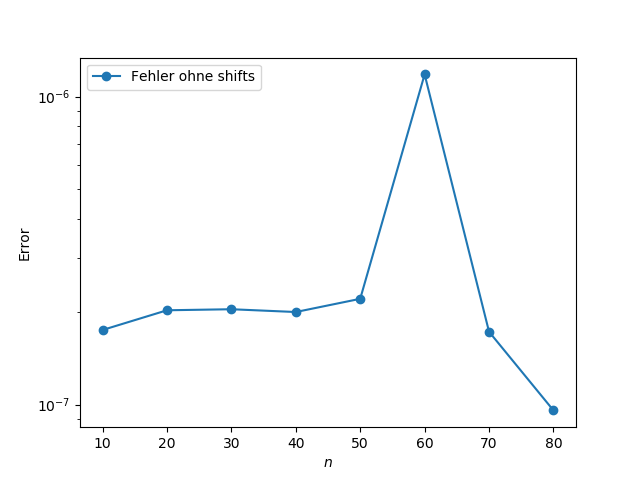
\includegraphics[width=0.45\linewidth]{Plots/error_wo_shifts}}%
  \qquad
  \subfloat[][Mit shifts]{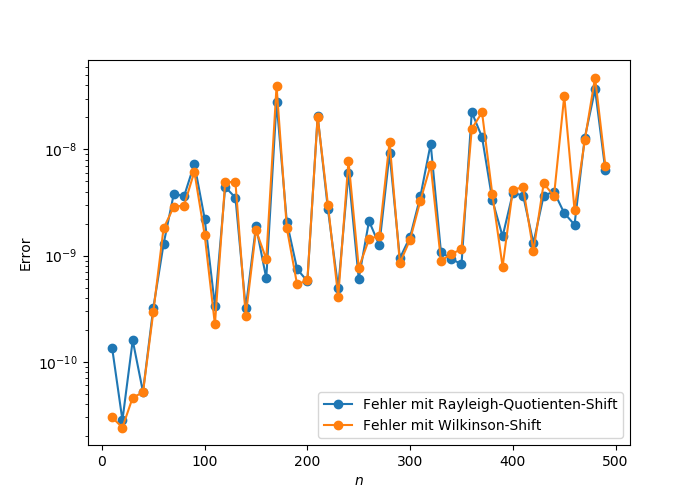
\includegraphics[width=0.45\linewidth]{Plots/error_shifts}}%
  \caption{Fehler in den Eigenwerten, gemessen in $||\cdot||_2$ bei Matrixdimension $n$}%
  \label{Error_QR}
\end{figure}

\section{Das Lanczos-Verfahren}
Wie in der Einleitung erwähnt, liefert uns das dort beschriebene Eigenwertproblem Matrizen mit sehr großer Dimension. Außerdem ist man in der Praxis häufig nur an wenigen extremalen Eigenwerten interessiert. Das QR-Verfahren ist für solche Probleme also nicht geeignet. Im Folgenden werden wir deshalb das Lanczos-Verfahren kennenlernen.

\subsection{Idee}

Wir zeigen zunächst ein theoretisches Resultat, welches eine Darstellung der Eigenwerte für hermitesche Matrizen liefert. Man sieht leicht, dass es sich hierbei um eine Verallgemeinerung des Satzes von Rayleigh handelt.

\begin{lemma} \label{Rayleigh}
	Sei $A \in \C^{n \times n}$ hermitesch bezüglich des Skalarproduktes $(\cdot, \cdot)$, $\lambda_1 \geq \lambda_2 \geq \dots \geq \lambda_n$ die Eigenwerte von $A$ (gemäß Vielfachheit gezählt) und $u_1, \dots, u_n$ die zugehörigen normierten Eigenvektoren. Dann gilt
	\begin{align}\label{lambdamax}
		\lambda_1 = \max_{v \in \C^n \setminus \{0\}} \frac{(Av,v)}{(v,v)}, \quad \lambda_k = \max_{\substack{v \in \C^n \setminus \{0\}\\
    (u_j,v) = 0, j= 1,\dots, k-1}} \frac{(Av,v)}{(v,v)}, \quad k= 2, \dots, n
	\end{align}
	und
	\begin{align}\label{lambdamaxmin}
		\lambda_k = \max_{\substack{S \subset \C^n\\
    \dim S = k}} \min_{v \in S \setminus \{0\}} \frac{(Av,v)}{(v,v)}, \quad k=1, \dots n.
	\end{align}

	Für $v \neq 0$ nennt man $\frac{(Av,v)}{(v,v)}$ den Rayleigh-Quotienten von $v$.
\end{lemma}

\begin{proof}
	Sei $v \in \C^n \setminus \{0\}$ beliebig. Da $u_1, \dots, u_n$ eine Orthonormalbasis des $\C^n$ bilden, gilt $ v = \sum_{j=1}^{n} (v,u_j) u_j$ und $\|v\|^2 = \sum_{j=1}^{n} |(u_j,v)|^2$. Damit folgt
	\begin{align*}
		(Av,v) = \sum_{j=1}^{n} (v,u_j) (\lambda_j u_j,v) = \sum_{j=1}^{n} \lambda_j |(u_j,v)|^2 \leq \lambda_1 \sum_{j=1}^{n} |(u_j,v)|^2 = \lambda_1 (v,v).
	\end{align*}
	Dividieren durch $(v,v)$ liefert $\lambda_1 \geq \frac{(Av,v)}{(v,v)}$ für alle $v \in \C^n \setminus \{0\}$ und für $v = u_1$ gilt sogar Gleichheit.

	Für ein anderes $k = 2,\dots,n$ können wir analog ein beliebiges $v \in \C^n \setminus \{0\}$ wählen, nun aber mit der Bedingung $(u_j,v) = 0, j=1,\dots,k$ betrachten. In der Summe $\sum_{j=1}^{n} \lambda_j |(u_j,v)|^2$ fallen somit die ersten $k-1$ Summanden weg und wir können die verbleibenden Eigenwerte mit $\lambda_k$ nach oben abschätzen. Gleichheit gilt für den jeweiligen Eigenvektor $u_k$.

	Für die Gleichheit in \ref{lambdamaxmin} gilt ähnlich zu oben für $v \in \tilde{S} := \textbf{span}\{v_1, \dots, v_k\}$, dass
	\begin{align*}
		(Av,v) = \sum_{j=1}^{k} \lambda_j |(v,u_j)|^2 \geq \lambda_k (v,v)
	\end{align*}

	und daraus $\lambda_k \leq \min_{v \in \tilde{S}} \frac{(Av,v)}{(v,v)}$. Für $v = u_k$ gilt wiederum Gleichheit.

	Betrachten wir nun einen anderen Unterraum $S \neq \tilde{S}$ mit $\dim S = k$. Dann gibt es ein $v_0 \in S \setminus \{0\}$ mit $(v_0,u_j) = 0$ für $j=1,\dots,k$. Für dieses $v_0$ gilt $(Av_0,v_0) \leq \lambda_k (v_0,v_0)$. Das heißt, für beliebige solche $S$ ist $\min_{v \in S \setminus \{0\}} \frac{(Av,v)}{(v,v)} \leq \lambda_k$, womit die Gleichheit gezeigt ist.
\end{proof}

Wir wollen das Verfahren der Vektoriteration zur Bestimmung des größten Eigenwertes einer hermiteschen Matrix wiederholen. Diese erzeugt ausgehend von einem Startvektor $x^{(0)} \in \C^{n}$ eine Folge von Iterierten $x^{(m)} := \frac{Ax^{(m-1)}}{\|Ax^{(m-1)}\|}$ für $m \in \N$. Definiert man die Approximationen $\lambda^{(m)}$ an den größten Eigenwert $\lambda_1$ durch den Rayleigh-Quotienten von $x^{(m-1)}$, so konvergiert $\lambda^{(m)}$ quadratisch gegen $\lambda_1$. (vgl.\ \cite{Num}, Satz 9.9)

\begin{definition}[Krylov-Raum]
	Sei $v_0 \in \C^{n}$ und $A \in \C^{n \times n}$. Dann bezeichnet
	\begin{align*}
		\mathcal{K}_m(A,v_0) := \textbf{span}\{v_0, Av_0, \dots, A^{m-1}v_0\}, \quad m \in \N
	\end{align*}
	den Krylov-Raum von $A$ und $v_0$. Es bezeichne $\mathcal{P}_m \in \C^{n \times n}$ die orthogonale Projektion auf $\mathcal{K}_m$, also die eindeutige hermitesche Matrix mit $\mathcal{P}_m^2 = \mathcal{P}_m$ und $\mathcal{R}(\mathcal{P}_m) = \mathcal{K}_m$.
\end{definition}

Beim Lanczos-Verfahren wird nun als Näherung an den größten Eigenwert das Maximum des Rayleigh-Quotienten über dem Krylov-Raum
\begin{align*}
	\mathcal{K}_m(A,x^{(0)}) = \textbf{span}\{x^{(0)}, x^{(1)}, \dots , x^{(m-1)} \}
\end{align*}
verwendet, also

\begin{align*}
	\lambda_1^{(m)} := \max_{x \in \mathcal{K}_m \setminus \{0\}} \frac{(Ax,x)}{(x,x)}.
\end{align*}

Da $x^{(t-1)} \in \mathcal{K}_m$, gilt
\begin{align*}
	\lambda^{(m)} \leq \lambda_1^{(m)} \leq \lambda_1
\end{align*}

und $\lambda_1^{(m)}$ ist somit eine mindestens so gute Approximation von $\lambda_1$ wie $\lambda^{(m)}$.

Betrachten wir die Abbildung

\begin{align*}
	\mathcal{A}_m: \mathcal{K}_m &\to \mathcal{K}_m \\
	x &\mapsto \mathcal{P}_m Ax,
\end{align*}

so sehen wir, dass diese selbstadjungiert ist. Es gilt für $x,y \in \mathcal{K}_m$

\begin{align*}
	(\mathcal{A}_mx, y) = (\mathcal{P}_m A \mathcal{P}_m x, y) = (x, \mathcal{P}_m A \mathcal{P}_m y) = (x, \mathcal{A}_m y),
\end{align*}

da $\mathcal{P}_m$ und $A$ hermitesch sind. Also besitzt $ \mathcal{A}_m$ nur reelle Eigenwerte $\lambda_1(\mathcal{A}_m) \geq \lambda_2(\mathcal{A}_m) \geq \dots \geq \lambda_m(\mathcal{A}_m)$. Für den größten Eigenwert gilt

\begin{align*}
	\lambda_1(\mathcal{A}_m) = \max_{x \in \mathcal{K}_m \setminus \{0\}} \frac{(x, \mathcal{A}_m x)}{(x,x)} = \max_{x \in \mathcal{K}_m \setminus \{0\}} \frac{(\mathcal{P}_m x, A x)}{(x,x)} = \max_{x \in \mathcal{K}_m \setminus \{0\}} \frac{(x, A x)}{(x,x)} = \lambda_1^{(m)}.
\end{align*}

Die erste Gleichheit kann man sich mit gleichen Rechnungen wie im Beweis von Lemma \ref{Rayleigh} überlegen. Der größte Eigenwert $\lambda_1(\mathcal{A}_m)$ von $\mathcal{A}_m$ ist also nach unseren bisherigen Überlegungen eine gute Approximation an den größten Eigenwert $\lambda_1$ von $A$. Es liegt nahe, für alle $j \leq m$ auch $\lambda_j(\mathcal{A}_m)$ als Approximation von $\lambda_j$ zu betrachten. Dass dies eine gute Wahl ist, werden wir im übernächsten Unterabschnitt zeigen.

\subsection{Herleitung des Verfahrens}

Im Vertrauen auf die Sinnhaftigkeit der eben gemachten Überlegungen ist es also nun Ziel, die Eigenwerte der Abbildung $\mathcal{A}_m$ zu berechnen. Hierfür benötigen wir eine Repräsentation von $\mathcal{A}_m$ durch eine Matrix $T_m$ bezüglich einer Orthonormalbasis $\{v_0, \dots, v_{m-1}\}$ des Krylov-Raums $\mathcal{K}_m(A,v_0)$. Für die Einträge von $T_m$ gilt
\begin{align*}
	(T_m)_{ij} &= (v_i, \mathcal{A}_m v_j) = v_i^*Av_j \\
	\Rightarrow T_m &= V_m^*AV_m.
\end{align*}

Der Vorteil dieser Darstellung ist, dass die Eigenwerte von $T_m$ jenen von $\mathcal{A}_m$ entsprechen. Wenn wir $m$ nicht zu groß gewählt haben, können wir diese mit dem aus Kapitel 2 bekannten QR-Verfahren mit wenig Aufwand berechnen.

Eine Möglichkeit zur Bestimmung einer Orthonormalbasis liefert das CG-Verfahren, auf welches an dieser Stelle nicht genauer eingegangen werden soll. Aus diesem ergibt sich der Ansatz, $T_m$ als eine Tridiagonalmatrix (also auch Hessenbergmatrix) der Form

\begin{align}\label{trimatrix}
\begin{pmatrix}
	\gamma_0 & \delta_0 & 0 & \hdots & 0 \\
	\delta_0 & \gamma_1 & \delta_1 &  & \vdots \\
	0 & \delta_1 & \ddots & \ddots & 0 \\
	\vdots &  & \ddots & \ddots & \delta_{m-2} \\
	0 & \hdots & 0 & \delta_{m-2} & \gamma_{m-1}
\end{pmatrix}
\end{align}

aufzustellen. Die Gleichung **ref** schreiben wir um als $AV_m = V_m T_m$, was spaltenweise zu folgenden Gleichungen führt:
\begin{align*}
	A v_0 &= \gamma_0 v_0 + \delta_0 v_1 \\
	A v_j &= \delta_{j-1} v_{j-1} + \gamma_j v_j + \delta_j v_{j+1}, \quad j=1, \dots, m-2.
\end{align*}

Da es sich bei $\{v_0, \dots, v_{m-1}\}$ um ein Orthogonalsystem handelt, liefert Multiplizieren der $j$-ten Gleichung von links mit $v_j^*$ die Bedingung $\gamma_j = v_j^*Av_j$ für $j = 0, \dots, m-2$. Somit können wir die $j$-te Gleichung rekursiv nach $v_{j+1}$ auflösen:

\begin{align*}
	v_{j+1} = \begin{cases}
		\frac{\overbrace{(A-\gamma_0)v_0}^{=:w_0}}{\delta_0} &,j = 0 \\
		\frac{\overbrace{(A-\gamma_j)v_j - \delta_{j-1} v_{j-1}}^{=:w_j}}{\delta_j} &,j \geq 1
	\end{cases}
\end{align*}

Hierbei setzen wir $\delta_j := \|w_j\|$ falls $\|w_j\| \neq 0$. Andernfalls bricht die Iteration ab. Daraus ergibt sich nun der Algorithmus für das Lanczos-Verfahren.

\renewcommand{\algorithmicrequire}{\textbf{Input:}}
\renewcommand{\algorithmicensure}{\textbf{Output:}}

\begin{algorithm}
	\label{Lanczos-Verfahren}
	\caption{Lanczos-Verfahren}
	\algorithmicrequire{ $A \in \C^{n\times n}$ hermitesche Matrix, zufälliger normierter Startvektor $v_0 \in \C^n$, maximale Krylov-Raum-Dimension $m$}
	\begin{algorithmic}[1]
		\State $\gamma_0 = v_0^*Av_0$
		\State $w_0 = (A-\gamma_0 I)v_0$
	  \State $\delta_0 = \|w_0\|_2$
		\While{$\delta_j \neq 0$ und $j < m$}
		\State $v_{j+1} = w_j/\delta_j$
		\State $j = j+1$
		\State $\gamma_j = v_j^*Av_j$
		\State $w_j = (A-\gamma_j I)v_j - \delta_{j-1}v_{j-1}$
		\State $\delta_j = \|w_j\|_2$
		\EndWhile
		\State Berechne mittels QR-Verfahren Eigenwerte von $T_j \in \C^{j \times j}$ aus \ref{trimatrix} (Hessenbergmatrix)
	\end{algorithmic}
	\algorithmicensure{Approximation an die Eigenwerte von $\mathcal{A}_j$}
\end{algorithm}


\subsection{Konvergenz der Eigenwerte von hermiteschen Matrizen}

In diesem Abschnitt beweisen wir, dass die durch das Lanczos-Verfahren erhaltenen Eigenwerte $\lambda_1^{(m)},\dots,\lambda_m^{(m)}$ gegen Eigenwerte $\lambda_1,\dots,\lambda_m$ der hermiteschen Matrix $A \in \C^{n \times n}$ konvergieren. Die Argumentation ist dabei in großen Teilen angelehnt an \cite{EWPs}, Abschnitt 4.1.

Wir werden ein Lemma benötigen, welches Elemente des Krylov-Raums in Zusammenhang mit Polynomen charakterisiert.

\begin{lemma}
	\label{v0_Polynom_Darstellung}
	Sei $\Pi_m$ der Raum der Polynome in einer Veränderlichen mit maximalem Grad $m$. Dann ist $v \in \mathcal{K}_m(A,v_0) \subset \C^n$ genau dann, wenn ein Polynom $p \in \Pi_{m-1}$ existiert mit $v = p(A)v_0$. \newline
	Ist $A$ diagonalisierbar mit Eigenwerten $\lambda_1, \dots, \lambda_n$ und zugehörigen Eigenvektoren $u_1, \dots, u_n$, dann existiert eine eindeutige Darstellung $v_0 = \sum_{j=1}^{n} \alpha_j u_j$ und es gilt
	\begin{align*}
		v \in \mathcal{K}_m \Leftrightarrow \Exists p \in \Pi_{m-1}: v = \sum_{j=1}^{n} p(\lambda_j)\alpha_j u_j.
	\end{align*}
\end{lemma}

\begin{proof}
	Wir zeigen zunächst die erste Aussage. Nach Definition des Krylov-Raums gilt
	\begin{align}
		v \in \mathcal{K}_m \Leftrightarrow& \Exists a_0, \dots a_{m-1} \in \C: v = \sum_{i=0}^{m-1} a_i A^i v_0 = (\sum_{i=0}^{m-1} a_i A^i)v_0\\
		\Leftrightarrow& \Exists p(x) = \sum_{i=0}^{m-1} a_i x^i \in \Pi_{m-1}: v = p(A)v_0.
		\label{eq:Krylov}
	\end{align}

	Da die Eigenvektoren eine Basis des $\C^n$ bilden, folgt die eindeutige Darstellung von $v_0$. Setzen wir diese in die erste Zeile von \ref{eq:Krylov} ein und verwenden die Tatsache, dass $A^i u_j = \lambda_j^i u_j$ für $j=1,\dots, n $ und $i = 0, \dots, m-1$, erhalten wir auch die zweite Aussage.
\end{proof}


\begin{definition}
	Für $m \in \N$ sind die Chebyshev-Polynome $T_m \in \Pi_m$ definiert durch
	\begin{align}\label{chebyshev}
		T_m(x) := \frac{1}{2}((x+ \sqrt{x^2 - 1})^m + (x- \sqrt{x^2 - 1})^m), \quad x \in \R.
	\end{align}
\end{definition}

Es gibt weitere Definitionen der Chebyshev-Polynome. Die Bekannteste ist
\begin{align}\label{chebyalt}
	T_m(x) := \cos(m \arccos x), \quad x \in [-1,1],
\end{align}

welche aus der Identität $T_m(\cos \varphi) = \cos (m \varphi)$ für $\varphi \in \R$ folgt.

Aus dieser Darstellung folgt auch mittels Additionstheorem die 2-Term-Rekursion

\begin{align*}
	T_0(x) = 1, \quad T_1(x) = x, \quad T_{m}(x) = 2x T_{m-1}(x) - T_{m-2}(x), \quad m \geq 2,
\end{align*}

welche zeigt, dass es sich bei $T_m$ tatsächlich um ein Polynom vom Grad $m$ handelt.

\begin{lemma}
	\label{lem:polminmax}
	Sei $[a,b]$ ein nicht-leeres Intervall in $\R$ und sei $c \geq b$. Dann gilt mit $\gamma := 1 + 2 \frac{c-b}{b-a} \geq 1$
	\begin{align}\label{polminmax}
		\min_{\substack{p \in \Pi_m \\
		p(c) = 1}} \max_{x \in [a,b]} |p(x)| \leq \frac{1}{|T_m(\gamma)|} \leq 2 (\gamma + \sqrt{\gamma^2 -1})^{-m}.
	\end{align}
\end{lemma}

\begin{proof}
	Wir verwenden die affin lineare Abbildung $\Phi: [a,b] \to [-1,1]$ mit
	\begin{align*}
		\Phi(x) = 1 + 2 \frac{x-b}{b-a}, \quad x \in [a,b].
	\end{align*}
	Wir definieren
	\begin{align*}
		\hat{p} := \frac{T_m \circ \Phi}{|T_m(\Phi(c))|}
	\end{align*}
	und können die Darstellung von $T_m$ aus \ref{chebyalt} verwenden (da $\Phi$ nach $[-1,1]$ abbildet), aus der
	\begin{align*}
		\max_{x \in [a,b]}|\hat{p}(x)| \leq \frac{1}{|T_m(\gamma)|}
	\end{align*}
	folgt und daraus auch die erste Ungleichung.

	Die zweite Ungleichung folgt aus der Definition der Chebyshev-Polynome \ref{chebyshev} und der Tatsache, dass $\gamma \geq 1$ und deshalb $|T_m(\gamma)| = T_m(\gamma) \geq \frac{1}{2} (\gamma+ \sqrt{\gamma^2-1})^m$ gilt.
\end{proof}

Mit den bis hier getroffenen Vorbereitungen können wir nun die Konvergenz des Projektionsverfahrens nachweisen.

\begin{theorem}[Konvergenz der Eigenwerte hermitescher Matrizen]
	Sei $A \in \C^{n \times n}$ eine hermitesche Matrix mit paarweise verschiedenen Eigenwerten $\lambda_1 > \lambda_2 > \dots > \lambda_n$. Bezeichne mit $u_1,\dots,u_n$ eine Orthonormalbasis aus Eigenvektoren zu den jeweiligen Eigenwerten. Für $1 \le m < n$ werden die Eigenwerte der linearen Abbildung $\mathcal{A}_m: \mathcal{K}_m(A,v_0)\rightarrow \mathcal{K}_m(A,v_0)$, die durch $v \mapsto \mathcal{P}_mAv$ gegeben ist,  mit $\lambda_1^{(m)} \ge \lambda_2^{(m)} \ge \dots \ge \lambda_m^{(m)}$ bezeichnet. Dabei ist $v_0$ ein beliebiger Startvektor, der nicht orthogonal zu den ersten $m-1$ Eigenvektoren von $A$ ist. Dann gilt

	\begin{equation}
		\label{konvergenz Eigenwerte}
		0 \le \lambda_i - \lambda_i^{(m)} \le (\lambda_i -\lambda_n) (\tan\theta_i)^2 \kappa_i^{(m)} \left(\frac{1}{T_{m-i}(\gamma_i)}\right)^2, \quad i=1,\dots,m-1,
	\end{equation}

	wobei
	\begin{equation*}
		\tan \theta_i \coloneqq \frac{\norm{(\id - \mathcal{P}_{u_i})v_0}}{\norm{ \mathcal{P}_{u_i}v_0}}, \quad \gamma_i \coloneqq 1+2 \frac{\lambda_i-\lambda_{i+1}}{\lambda_{i+1} -\lambda_n}
	\end{equation*}

	und
	\begin{equation*}
		\kappa_1^{(m)} \coloneqq 1, \quad \kappa_i^{(m)} \coloneqq \left(\prod_{k=1}^{i-1} \frac{\max_{j=i+1,\dots,n} (\lambda_k^{(m)} - \lambda_j)}{\lambda_k^{(m)} - \lambda_i}\right)^2, \quad i = 2,\dots,m.
	\end{equation*}

	Dabei wird mit $\mathcal{P}_{u_i}$ die Projektion auf den eindimensionalen Unterraum, der von $u_i$ aufgespannt wird, bezeichnet. Das $\theta_i$ kann somit als Winkel zwischen $v_0$ und $u_i$  verstanden werden.
	\begin{proof}

	Seien $v_1, \dots, v_m$ Orthonormalbasisvektoren von $\mathcal{K}_m$ und $V \in \C^{n\times m}$ die Matrix, die diese Vektoren als Spalten besitzt. Dann ist

	\begin{equation*}
		T_m \coloneqq V^* A V \in \C^{m\times m}
	\end{equation*}

	die Matrixdarstellung der Abbildung $\mathcal{A}_m$ bezüglich der Orthonormalbasis $\{v_1,\dots,v_m\}$.

	Diese Matrix ist offensichtlich hermitesch. Somit können die Eigenwerte $\lambda_1^{(m)}, \dots, \lambda_m^{(m)}$ mithilfe von \eqref{lambdamaxmin} berechnet werden.

	Es gilt also

	\begin{equation}
		\label{Eigenwert_Ungl}
		\begin{aligned}
			\lambda_k^{(m)} &= \max_{\substack{S \subseteq \C^m\\ \dim S = k}} \min_{v\in S\setminus\{0\}} \frac{(T_m v,v)}{(v,v)} \\
			&= \max_{\substack{S \subseteq \C^m\\ \dim S = k}} \min_{v\in S\setminus\{0\}} \frac{(AVv,Vv)}{(Vv,Vv)}\\
			&= \max_{\substack{T \subseteq \mathcal{K}_m \\ \dim T = k}} \min_{w\in T\setminus\{0\}} \frac{(Aw,w)}{(w,w)}\\
			 &\le \max_{\substack{T \subseteq \C^n\\ \dim T = k}} \min_{w\in T\setminus\{0\}} \frac{(Aw,w)}{(w,w)} = \lambda_k.
		\end{aligned}
	\end{equation}

	Dabei gilt die dritte Gleichheit, da $V$ als Abbildung von $\C^m$ nach $\mathcal{K}_m$ bijektiv ist. Also kann jeder $k$-dimensionale Unterraum $T \subseteq \mathcal{K}_m$ als Bild von einem $k$-dimensionalen Unterraum $S \subseteq \C^m$ mit der Abbildung $V$ gesehen werden.
	Somit ist die erste Ungleichung in \eqref{konvergenz Eigenwerte} erfüllt.\\

	Wir beweisen nun die zweite Ungleichung zuerst für den Fall $i = 1$.
	Sei $v_0 = \sum_{j=1}^{n}\alpha_j u_j$. Wir bemerken, dass $\alpha_1, \dots, \alpha_{m-1}$ nicht verschwinden, da $v_0$ nicht orthogonal zu diesen Eigenvektoren gewählt wurde. Dies Rechtfertigt im folgenden Abschätzungen, bei denen ohne diese Bedingung durch Null geteilt werden würde.\\

	Mit analogen Umformungen wie in \eqref{Eigenwert_Ungl}, dem Satz von Pythagoras und Lemma \ref{v0_Polynom_Darstellung} gilt somit
	\begin{equation}
		\label{Ungl i=1}
		\begin{aligned}
			\lambda_1 - \lambda_1^{(m)} &= \lambda_1 - \max_{v \in \mathcal{K}_m \setminus\{0\}} \frac{(Av,v)}{(v,v)} = \min_{v \in \mathcal{K}_m\setminus\{0\}} \lambda_1 - \frac{(Av,v)}{(v,v)} = \min_{v \in \mathcal{K}_m\setminus\{0\}} \frac{\lambda_1(v,v) - (Av,v)}{(v,v)} \\ &= \min_{p\in \Pi_{m-1}\setminus \{0\}} \frac{\lambda_1 \norm{\sum_{j=1}^{n}p(\lambda_j)\alpha_j u_j}^2 - (\sum_{j=1}^{n}p(\lambda_j)\alpha_j A u_j,\sum_{j=1}^{n}p(\lambda_j)\alpha_j u_j)}{\norm{\sum_{j=1}^{n}p(\lambda_j)\alpha_j u_j}^2} \\
			&= \min_{p\in \Pi_{m-1}\setminus \{0\}} \frac{\lambda_1 \sum_{j=1}^{n} |p(\lambda_j)\alpha_j|^2 - \sum_{j=1}^{n} \lambda_j |p(\lambda_j)\alpha_j|^2 }{\sum_{j=1}^{n} |p(\lambda_j)\alpha_j|^2} \\
			&\le \min_{\substack{p\in \Pi_{m-1} \\ p(\lambda_1) =1}} \frac{\sum_{j=2}^{n} (\lambda_1 - \lambda_j)|p(\lambda_j)\alpha_j|^2}{\sum_{j=1}^{n} |p(\lambda_j)\alpha_j|^2} \\
			&\le (\lambda_1 - \lambda_n) \frac{\sum_{j=2}^{n} |\alpha_j|^2}{|\alpha_1|^2} \min_{\substack{p\in \Pi_{m-1} \\ p(\lambda_1) =1}} \max_{j=2,\dots,n} \left(\frac{|p(\lambda_j)|}{|p(\lambda_1)|}\right)^2.
		\end{aligned}
	\end{equation}

	Wir betrachten nun den Ausdruck $\tan \theta_i$. Dieser entspricht wegen
		\begin{equation*}
			(\tan\theta_1)^2 = \frac{\norm{(\id - \mathcal{P}_{u_1})v_0}^2}{\norm{ \mathcal{P}_{u_1}v_0}^2} = \frac{\norm{v_0 - \alpha_1 u_1}^2}{\norm{\alpha_1 u_1}^2} = \frac{\sum_{j=2}^{n} |\alpha_j|^2}{|\alpha_1|^2}
		\end{equation*}
	genau einem Term, der in obiger Abschätzung vorkommt.
	Mithilfe der Ungleichung \eqref{polminmax} mit $a = \lambda_n, b= \lambda_2$ und $c= \lambda_1$ erhalten wir außerdem

		\begin{equation*}
			\min_{\substack{p\in \Pi_{m-1} \\ p(\lambda_1) = 1}} \max_{j=2,\dots,n} 	\left(\frac{|p(\lambda_j)|}{|p(\lambda_1)|}\right)^2 \le \min_{\substack{p\in \Pi_{m-1} \\ p(\lambda_1) = 1}} \max_{\lambda \in [\lambda_n,\lambda_2]} |p(\lambda)|^2 \le \left(\frac{1}{T_{m-1}(\gamma_1)}\right)^2.
		\end{equation*}
	Daraus folgt die gewünschte Ungleichung und \eqref{konvergenz Eigenwerte} ist für $i = 1$ erfüllt.\\

	Betrachten wir nun den Fall $i>1$.
	Bezeichne mit $u_j^{(m)} \in \C^m, \, j = 1,\dots, m$ eine Orthonormalbasis aus Eigenvektoren zu den Eigenwerten $\lambda_j^{(m)} , \, j = 1,\dots, m$ der Abbildung $T_m$. Mit \eqref{lambdamax} erhalten wir dann

	\begin{equation}
		\begin{aligned}
			\label{Darstellung EW}
			\lambda_i^{(m)} &= \max_{\substack{v\in \C^n\setminus \{0\} \\ (u_j^{(m)},v) = 0, j = 1,\dots,i-1}} \frac{(A^{(m)}v,v)}{(v,v)} \\
			&= \max_{\substack{v\in \C^n\setminus \{0\} \\ (u_j^{(m)},v) = 0, j = 1,\dots,i-1}} \frac{(AVv,Vv)}{(Vv,Vv)}\\
			&= \max_{\substack{w\in \mathcal{K}_m\setminus \{0\} \\ (Vu_j^{(m)},w) = 0 j = 1,\dots,i-1}} \frac{(Aw,w)}{(w,w)}
		\end{aligned}
	\end{equation}

	Da die $u_j^{(m)}, j = 1,\dots,m$ eine Orthonormalbasis von $\C^m$ sind, sind somit die $\tilde{u}_j^{(m)} \coloneqq \nicefrac{Vu_j^{(m)}}{\norm{Vu_j^{(m)}}}$ eine Orthonormalbasis von $\mathcal{K}_m$. Sei nun $w\in \mathcal{K}_m$ gegeben durch $w = \sum_{k=1}^{m} p(\lambda_k^{(m)}) \beta_k \tilde{u}_k^{(m)}$. Dann gilt für alle $j < i$
	\begin{equation*}
		0 \stackrel{!}{=} (w,\tilde{u}_j^{(m)}) = (\sum_{k=1}^{m} p(\lambda_k^{(m)}) \beta_k \tilde{u}_k^{(m)},\tilde{u}_j^{(m)}) = \sum_{k=1}^{m} p(\lambda_k^{(m)}) \beta_k (\tilde{u}_k^{(m)},\tilde{u}_j^{(m)}) = p(\lambda_j^{(m)}) \beta_j.
	\end{equation*}

	Es gibt also zwei Möglichkeiten, diese Gleichheit zu erfüllen. Entweder ist $p(\lambda_j^{(m)}) = 0$ oder $\beta_j = 0$. Wir betrachten zuerst den Fall, dass  $\beta_j \neq 0$ für alle $j = 1,\dots, i-1$ gilt.

	Da dann die $\lambda_j^{(m)}, \, j = 1,\dots,i-1$ Nullstellen von $p$ sind, können wir

	\begin{equation*}
		p(\lambda) = \prod_{j = 1}^{i-1} \frac{\lambda_j^{(m)} -\lambda}{\lambda_j^{(m)} - \lambda_i} q(x)
	\end{equation*}
	schreiben, wobei $q \in \Pi_{m-i}$.\\

	Mit der Darstellung \eqref{Darstellung EW} von $\lambda_i^{(m)}$ gilt nach analogen Umformungen wie in \eqref{Ungl i=1}

	\begin{equation*}
		\begin{aligned}
			\lambda_i - \lambda_i^{(m)} &= \min_{\substack{p\in \Pi_{m-1}\setminus \{0\} \\ p(\lambda_j^{(m)}) = 0, j = 1,\dots,i-1}} \frac{\sum_{j=1}^{n} (\lambda_i - \lambda_j)|p(\lambda_j)\alpha_j|^2}{\sum_{j=1}^{n} |p(\lambda_j)\alpha_j|^2} \\
			&= \min_{\substack{p\in \Pi_{m-1}\setminus \{0\} \\ p(\lambda_j^{(m)}) = 0, j = 1,\dots,i-1}} \frac{\sum_{\substack{j=1, j\neq i}}^{n} (\lambda_i - \lambda_j)|p(\lambda_j)\alpha_j|^2}{\sum_{j=1}^{n} |p(\lambda_j)\alpha_j|^2} \\
			& \le (\lambda_i - \lambda_n) \frac{\sum_{\substack{j=1, j\neq i}}^{n} |\alpha_j|^2}{|\alpha_i|^2} \min_{\substack{p\in \Pi_{m-1}, p(\lambda_i) \neq 0 \\ p(\lambda_j^{(m)}) = 0, j = 1,\dots,i-1}} \max_{j=i+1,\dots,n} \left(\frac{|p(\lambda_j)|}{|p(\lambda_i)|}\right)^2 \\
			&\le (\lambda_i - \lambda_n) \frac{\sum_{\substack{j=1, j\neq i}}^{n} |\alpha_j|^2}{|\alpha_i|^2} \min_{\substack{q\in \Pi_{m-i} \\ q(\lambda_i) = 1}} \max_{j=i+1,\dots,n} \left(\left|\prod_{k = 1}^{i-1} \frac{\lambda_k^{(m)} -\lambda_j}{\lambda_k^{(m)} - \lambda_i}\right| \left|\frac{q(\lambda_j)}{q(\lambda_i)}\right|\right)^2 \\
			&\le (\lambda_i - \lambda_n) \frac{\sum_{\substack{j=1, j\neq i}}^{n} |\alpha_j|^2}{|\alpha_i|^2} \left|\prod_{k = 1}^{i-1} \frac{\max_{j=i+1,\dots,n} (\lambda_k^{(m)} -\lambda_j)}{\lambda_k^{(m)} - \lambda_i}\right|^2 \min_{\substack{q\in \Pi_{m-i} \\ q(\lambda_i) = 1}} \max_{j=i+1,\dots,n} \left(\left|\frac{q(\lambda_j)}{q(\lambda_i)}\right|\right)^2. \\
		\end{aligned}
	\end{equation*}

	Wieder ist
	\begin{equation*}
		(\tan\theta_i)^2 = \frac{\norm{(\id - \mathcal{P}_{u_i})v_0}^2}{\norm{ \mathcal{P}_{u_i}v_0}^2} = \frac{\norm{v_0 - \alpha_i u_i}^2}{\norm{\alpha_i u_i}^2} = \frac{\sum_{\substack{j=1, j\neq i}}^{n} |\alpha_j|^2}{|\alpha_i|^2}
	\end{equation*}

	und  mit $a = \lambda_n, b= \lambda_{i+1}$, $c = \lambda_i$ in Lemma \ref{lem:polminmax}, erhalten wir die Behauptung.\\

	Wenn nun $\beta_j$ existieren, die gleich 0 sind, kann man die Bedinungung $p(\lambda_j^{(m)}) = 0$ für die Polynome, über die minimiert wird, weglassen.
	Da somit mehr Polynome betrachtet werden, wird das Minimum sicherlich nicht größer. Das heißt, wir können für diesen Fall die gleiche Abschätzung verwenden.
	Also gilt \eqref{konvergenz Eigenwerte} für alle $i = 1, \dots, m-1$.
	\end{proof}
\end{theorem}

Die mit $m$ exponentielle Konvergenz der Eigenwerte ist nun ersichtlich, da mit \eqref{polminmax}
\begin{equation*}
	\left(\frac{1}{T_{m-i}(\gamma_i)}\right)^2 \le 4 \left(\gamma_i + \sqrt{\gamma_i^2 -1}\right)^{-2(m-i)}
\end{equation*}
gilt. Die Konvergenzgeschwindigkeit nimmt in der Theorie in Richtung der kleineren Eigenwerte ab, da der Grad des Chebyshev-Polynoms mit wachsendem $i$ kleiner wird. Wir bemerken noch, dass bei der Approximation von $\lambda_i$ bei Eigenwerten $\lambda_i \approx \lambda_j, \, j < i$, das Produkt $\kappa_i^{(m)}$ groß werden kann, da der Nenner wegen $\lambda^{(m)}_j - \lambda_i$ klein wird. Dies hat eine schlechtere Approximation zur Folge. Die anderen vorkommenden Terme wie $\tan \theta_i$ oder auch der Zähler vom Produkt in $\kappa_i^{(m)}$ haben für die Größenordnung der Abschätzung eher wenig Bedeutung. Wie sich die Konvergenz in der Praxis verhält, wird in den nachfolgenden Abschnitten beschrieben.


\subsection{Implementierung und Arnoldi-Verfahren}

Die Implementation des Lanczos-Verfahrens entspricht dem Pseudocode und ist im Anhang zu finden. Hier werden wir besprechen, wo das Lanczos-Verfahren an seine Grenzen stößt. Da wir das Lanczos-Verfahren nur auf einfache Eigenwertprobleme und nicht auf verallgemeinerte Eigenwertprobleme der Form \ref{discretization} anwenden können, müssen wir so ein verallgemeinertes Eigenwertproblem zuerst nach Lemma \ref{lemma_1_3} zu einem äquivalenten einfachen Eigenwertproblem umformulieren. Hier kommt Bemerkung \ref{remark_1_4} zu tragen, das Lanczos-Verfahren können wir nicht ohne weiteres Anwenden.

Um diese Problematik zu umgehen werden wir das sogenannte Arnoldi-Verfahren verwenden. Auch in diesem Verfahren bekommen wir eine Orthonormalbasis des Kyrlov-Raums und eine Matrix, welche die Abbildung $\mathcal{A}_m$ bezüglich dieser Basis beschreibt. Dabei ist $\mathcal{A}_m$ nicht mehr selbstadjungiert. In dem Arnoldi-Verfahren wird nun jeder neue Basisvektor mit dem (modifizierten) Gram-Schmidtschen Orthogonalisierungsverfahren gewonnen. Dabei wird ein neuer Basisvektor zu allen bisherigen Basisvektoren orthogonalisiert. Dies ist ein wesentlicher unterschied zum Lanczos-Verfahren, wo nur gegen den vorhergegangenen Basisivektor orthogonalisiert werden musste.
Es macht Sinn auch beim Lanczos-Verfahren eine volle Reorthogonalisierung durchzuführen. Diese ist zwar etwas Aufwändiger, aber wenn nur gegen den vorherigen Basisvektor orthogonalisiert wird, kann es zu Auslöschung und somit zu Verlust der Orthogonalität kommen. Es gibt auch diverse Strategien, bei denen keine volle, sondern nur eine teilweise Reorthogonalisierung durchgeführt wird. Dazu gibt es eine vielzahl an Literatur, wir verweisen hier auf \cite{reorthogonalization}.

Die Matrix, die man schließlich aus dem Arnoldi-Verfahren erhält hat dann nicht Tridiagonalform sondern ist eine obere Hessenberg-Matrix. Die Eigenwerte dieser können wir wieder mit dem QR-Verfahren für Hessenberg-Matrizen approximieren.
Das Lanczos-Verfahren ist so gesehen eigenlich ein Spezialfall des Arnoldi-Verfahrens, es ist das Arnoldi-Verfahren angewandt auf hermitesche Matrizen.

Das Arnoldi-Verfahren funktioniert nun nicht nur für hermitesche Matrizen, sondern auch für allgemeine. Für einen Konvergenzbeweis des Arnoldi-Verfahrens verweisen wir auf \cite{Saad_book}. Im folgenden ist das Verfahren als Pseudocode formuliert.

\floatname{algorithm}{Algorithmus}
\renewcommand{\algorithmicrequire}{\textbf{Input:}}
\renewcommand{\algorithmicensure}{\textbf{Output:}}

\begin{algorithm}[H]

	\caption{Arnoldi-Verfahren}
	\label{Arnoldi-Verfahren}
	\algorithmicrequire{ $A \in \C^{n\times n}$, zufälliger normierter Startvektor $v_0 \in \C^n$}
	\begin{algorithmic}[1]
		\For{$j = 1,\dots,k$}
			\State $w = A v_{j-1}$
			\For{$l = 1, \dots, j$}
				\State $h_{l,j} = (w, v_{l-1})$
				\State $w = w - h_{l,j}v_{l-1}$
			\EndFor
			\State $h_{j+1,j} = \norm[2]{w}$
			\If{$h_{j+1,j} = 0$}
			\State Ein invarianter Unterraum wurde gefunden
			\Else
				\State $v_j = \frac{w}{h_{j+1,j}}$
			\EndIf
		\EndFor
	\end{algorithmic}
	\algorithmicensure{Die Vektoren $v_0,\dots,v_{k-1}$ bilden eine Orthonormalbasis des Kyrlov-Raums, die Matrix $H$ ist eine Hessenbergmatrix, die die Projektion von $A$ bezüglich dieser Basis darstellt}
\end{algorithm}


\subsection{Ergebnisse}

Zunächst wird das Lanczos-Verfahren mit zufällig generierten hermiteschen Matrizen mit bekannten Eigenwerten getestet. Dazu wird wieder ein zufälliges Array mit Eigenwerten generiert und die auf die Diagonalmatrix mit diesen Eigenwerten eine Ähnlichkeitstransformation, hier mit zufälligen unitäre Matrizen, angewendet. Dass dabei eine hermitesche Matrix entsteht, kann man schnell nachrechnen: Sei dazu $A \in \R^{n\times n}$ eine Diagonalmatrix und $B \in \C^{n\times n}$ eine unitäre Matrix. Dann gilt also für die aus der Ähnlichkeitstransformation entstehende Matrix

\begin{align*}
	B^{-1}AB
	=
	B^* A B
	\stackrel{!}{=}
	(B^* A B)^*
	=
	B^* A^* B^{**}
	=
	B^{-1} A B
\end{align*}
Erste Testungen mit zufällig generierten uniform Verteilten Eigenwerten zeigten sehr mäßige Konvergenz von sowohl den größten als auch den kleinsten Eigenwerten. In Abbildung \ref{error_uniform} ist der absolute Fehler in den 2 größten Eigenwerten für steigende Kyrlovraumdimension dargestellt.Dabei wurde das Lanczos-Verfahren auf eine Matrix der Dimension $1000$ mit Eigenwerten uniform Verteilt im Intervall $(-100,400)$ angewendet. Selbst bei Kyrlovraumdimension 100 haben wir noch keine gute Approximation an nur zwei Eigenwerte. Für uniform Verteilte Eigenwerte ist das Lanczos-Verfahren also nicht gut geeignet. Sobald jedoch Eigenwerte existieren, die sich weiter vom Spektrum entfernen, erhalten wir sehr schnelle Konvergenz gegen diese.

\begin{figure}[H]\label{error_uniform}
\begin{center}

	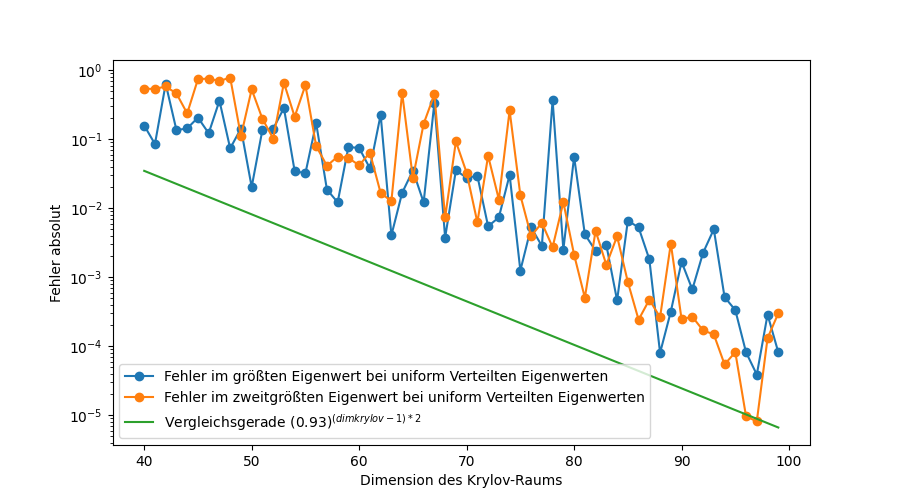
\includegraphics[width = 0.6 \linewidth]{Plots/error_uniform}
	\caption{Fehler im größten sowie zweitgrößten Eigenwert bei Verwendung des Lanczos-Verfahrens}
	\end{center}
\end{figure}

Diese Eigenschaft und andererseits die Symmetrie der Konvergenz kann man sehr gut in \ref{eigv_lanczos} erkennen. Dort wurde das Lanczos-Verfahren auf eine $500 \times 500$ Matrix, mit Eigenwerten gleichverteilt im Intervall $(0,2)$ und $4$ extremalen Eigenwerten bei $-1$, $-0.5$, $2.5$ und $3$, angewendet. Bei $x = 12$ sieht man das gesamte Spektrum der Eigenwerte, wobei ein Eigenwert durch ein Kreuz mit dem entsprechenden Wert an der $y-$Achse dargestellt wird. Für $x = 2,...,11$ sind die Approximationen an die Eigenwerte bei entsprechender Kyrlovraumdimension dargestellt. Der größte sowie kleinste Eigenwert werden hier schon bei Kyrlovraumdimension $6$ gut approximiert. Bei Kyrlovraumdimension $10$ beginnt die rapide Konvergenz der Approximation an den zweitgrößten sowie zweitkleinsten Eigenwert.


\begin{figure}[H]\label{eigv_lanczos}
	\begin{center}
		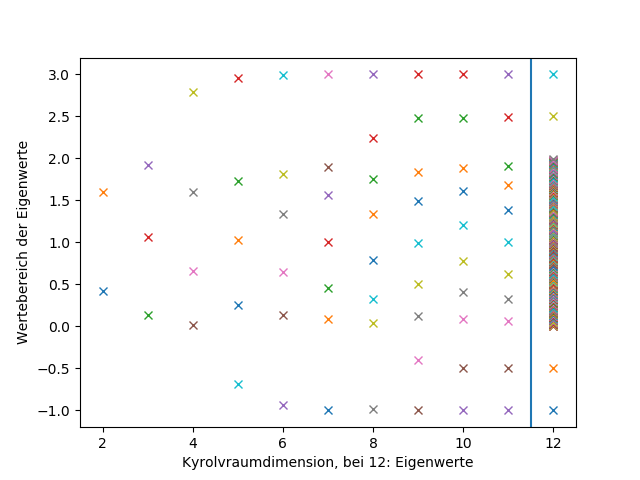
\includegraphics[width = 0.7 \linewidth]{Plots/eigv_kyrlov_approx}
		\caption{Die Approximation an die Eigenwerte beim Lanczos-Verfahren}
	\end{center}
\end{figure}



\begin{figure}[H]
\begin{center}
	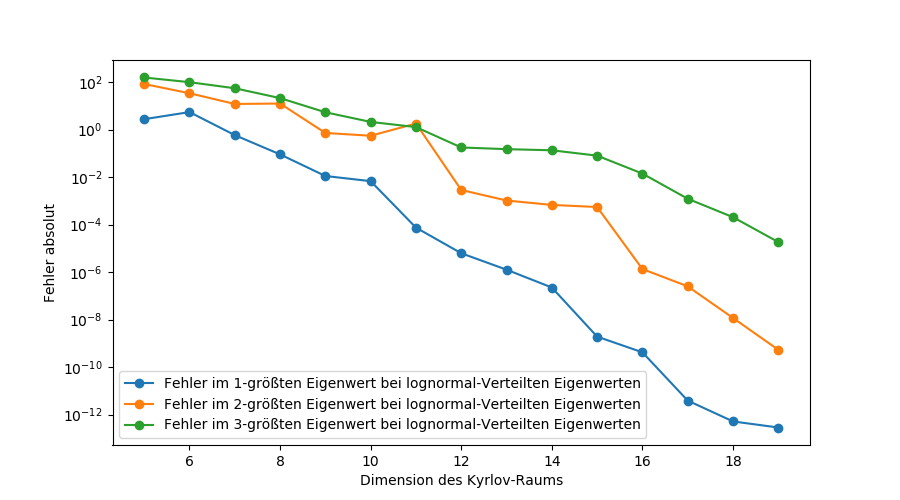
\includegraphics[width = 0.7 \linewidth]{Plots/lanczos_lognormal}\label{lanczos_lognomal}
	\caption{Fehler in den drei größten Eigenwerten bei Verwendung des Lanczos-Verfahrens mit lognormal-Verteilen Eigenwerten}
	\end{center}
\end{figure}

Verwenden wir nun also zur Testung keine uniform Verteilten Eigenwerte, sondern lognormal Verteilte erhalten wir nun wesentlich bessere Konvergenzgeschwindigkeit. In Abbildung \ref{lanczos_lognomal} wurde das Lanczos-Verfahren wieder auf eine Matrix der Dimension $1000$ angewendet, diesmal jedoch mit lognormal-Verteilen Eigenwerten ($\mu = 3, \sigma = 1$). Hier erkennt man die erwartete exponentielle Konvergenz, da der Fehler ja semilogarithmisch dargestellt wird.



Die Testungen zeigen also, dass sich das Lanczos-Verfahren vorallem für Eigenwertprobleme eignet, bei denen sich einige Eigenwerte stark vom Spektrum abheben. Beim Arnoldi-Verfahren erkennt man, bei Testung mit nun voll besetzten Matrizen, ein ähnliches Verhalten, auch hier kann man wesentlich bessere Konvergenzgeschwindigkeit bei lognormal-Verteilen Eigenwerten feststellen.

Wir wollen nun das Arnoldi-Verfahren verwenden, um unser Problem aus der Einleitung, die Eigenwertberechnung für $-\Delta$ auf einem Rechteck $\Omega$, zu lösen. Dabei verwenden wir zur Diskretisierung des Problems die Finite-Elemente-Methode. Hier kommen das Netgen sowie NG-Solve Paket zum Einsatz. Mit diesen können wir das Rechteck $\Omega := (0,2) \times (0,1)$ triangulieren und einen Finite-Elemente-Raum darauf erstellen. Aus NG-Solve bekommen wir dann unsere Matrizen. Zum Vergleich verwenden wir die in Satz \ref{satz_1_2} berechneten Eigenwerte. Als shift in \ref{equivdiscret} wurde $\rho = 3$ gewählt. In Abbildung \ref{error_eigv_laplace} sieht man den Fehler für verschiedene Kyrlovraumdimensionen. Dabei ist auf der $x-$Achse die Nummer des betrachteten Eigenwerts (aufsteigend sortiert) und auf der $y-$Achse je der Fehler von der Approximation aus dem Arnoldi-Verfahren zu dem analytisch berechneten Eigenwert. Wir erkennen eine gute Approximation in den ersten $40\%$ der berechneten Eigenwerte, wobei die Anzahl an berechneten Eigenwerten ja genau mit der Kyrlovraumdimension übereinstimmt. Die Schranke der $40\%$ wurde dabei aus Skalierungstechnischen Gründen gewählt, man erhält sogar eine ziemlich gute Approximation an die ersten (also kleinsten) $45\%$ Eigenwerte, bei den größeren steigt der Fehler jedoch schnell und stark an.

\begin{figure}\label{error_eigv_laplace}
	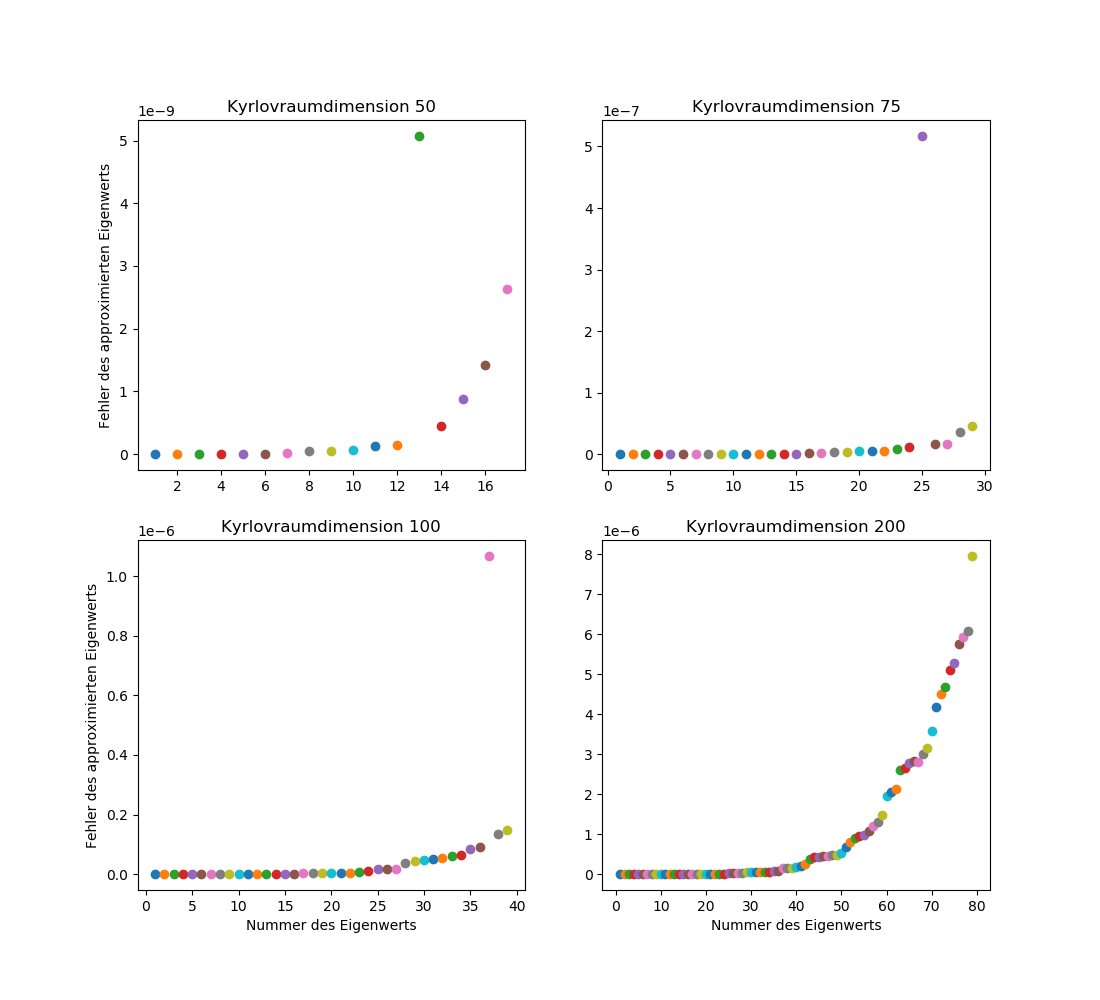
\includegraphics[width = 0.9\linewidth]{Plots/error_eigv_laplace}
	\caption{Fehler in den ersten 40\% der Eigenwerte bei Anwendung des Arnoldi-Verfahrens auf das diskretisierte Problem}
\end{figure}
\newpage
\pagestyle{plain}
\section*{Code}

\subsection*{QR-Verfahren ohne shifts}
\lstset{caption={Implementation des QR-Verfahren ohne shifts}}

\begin{lstlisting}
def QR_simple(A, tol = 1e-7):
	n = A.shape[1]
	count = 0
	for i in range(n-1,0,-1):
		while abs(A[i,i-1]) > tol:
				Q,R = np.linalg.qr(A)
				A = R@Q
				count +=1
		A[i,:i-n] = 0
return A, sorted(np.diag(A)), count
\end{lstlisting}



\subsection*{QR-Verfahren mit Rayleigh-Quotienten-Shift}
\lstset{caption={Implementation des QR-Verfahrens mit Rayleigh-Quotienten-Shift}}
\begin{lstlisting}
def QR_shift(A,tol=1e-10):
	n = A.shape[1]
	count = 0
	for i in range(n-1,0,-1):
			while abs(A[i,i-1]) > tol:
					rho = A[i,i]
					Q,R = np.linalg.qr(A-rho*np.identity(n))
					A = R@Q + rho*np.identity(n)
					count +=1
			A[i,:i-n] = 0
	return A, sorted(np.diag(A)), count
\end{lstlisting}


\subsection*{QR-Verfahren mit Wilkinson-Shift}

\lstset{caption={Implementation des QR-Verfahrens mit Rayleigh-Quotienten-Shift}}

\begin{lstlisting}
def QR_shift2(A,tol=1e-14):
    n = A.shape[1]
    count = 0
    for i in range(n-1,0,-1):
        while abs(A[i,i-1]) > tol*(abs(A[i-1,i-1])+abs(A[i,i])):
            w = np.linalg.eigvals(A[i-1:i+1,i-1:i+1])
            if abs(w[0] - A[i,i]) < abs(w[1] - A[i,i]):
                rho = w[0]
            else:
                rho = w[1]
            Q,R = np.linalg.qr(A-rho*np.identity(n))
            A = R@Q + rho*np.identity(n)
            count += 1
        A[i,:i-n] = 0
    return A, sorted(np.diag(A)), count
\end{lstlisting}

\subsection*{Lanczos-Verfahren}

\lstset{caption={Implementation des Lanczos-Verfahrens}}

\begin{lstlisting}
def lanczos(A,m = 0):
    n = A.shape[1]
    if m == 0:
        m = n

    v0 = np.random.rand(n)
    v = [v0/np.linalg.norm(v0)]
    gam = [v[0].T.conj()@A@v[0]]
    w = (A - gam[0]*np.identity(n))@v[0]
    delta = [np.linalg.norm(w)]
    j = 0
    while delta[j] > 1e-10 and j < m-1:
        v.append(w/delta[j])
        j +=1
        gam.append(v[j].T.conj()@A@v[j])
        w = (A - gam[j]*np.identity(n))@v[j] - delta[j-1]*v[j-1]
        delta.append(np.linalg.norm(w))
    T = np.diag(delta[:-1], -1) + np.diag(gam) + np.diag(delta[:-1], 1)
    return QR_hesse(T)
\end{lstlisting}

\subsection*{Arnoldi-Verfahren}

\lstset{caption ={Implementation des Arnoldi-Verfahrens}}

\begin{lstlisting}
def arnoldi(A, dim, k = 0):
	n = dim
	if k == 0:
			k = n

	v0 = np.random.rand(n)
	v = [v0/np.linalg.norm(v0)]
	h = np.zeros((k,k))

	for j in range(k):
			w = A(v[j])
			for l in range(j+1):
					h[l][j] = v[l].T.conj()@w
					w = w - h[l][j]*v[l]
			if j < k-1:
					h[j+1][j] = np.sqrt(w.T.conj()@w)
					if abs(h[j+1][j]) < 1e-14:
							return QR_hesse(h[:j+1,:j+1])
					else:
							v.append(w/h[j+1][j])
	return QR_hesse(h)
\end{lstlisting}
\newpage

\printbibliography

\end{document}
